
% VYSOKOŠKOLSKÁ KVALIFIKAČNÍ PRÁCE
% autor: Michal Struna
% název: Webový 3D simulátor těles ve vesmíru
% kódování zdroje: UTF-8

\documentclass[a4paper,12pt]{article}

\usepackage{vskpupa}	% globální nastavení pro text VŠKP UPa
\usepackage{listings}
\usepackage{geometry}
\def\code#1{\texttt{#1}}
\setlist{itemsep=0pt,topsep=2pt}
\renewcommand{\lstlistingname}{Zdrojový kód}
\renewcommand{\lstlistlistingname}{Seznam zdrojových kódů}

\expandafter\def\expandafter\UrlBreaks\expandafter{\UrlBreaks%  save the current one
  \do\-}

\let\oldlstlistoflistings\lstlistoflistings
\renewcommand{\lstlistoflistings}{%
  \begingroup%
  \let\oldnumberline\numberline%
  \renewcommand{\numberline}{\lstlistingname~\oldnumberline}%
  \oldlstlistoflistings%
  \endgroup}

\usepackage{color}
\definecolor{lightgray}{rgb}{.9,.9,.9}
\definecolor{darkgray}{rgb}{.4,.4,.4}
\definecolor{gray}{rgb}{0.6, 0.6, 0.6}

\titleformat{\section}
	{\Large\bfseries}
	{\thesection}
	{1em}
	{\MakeUppercase}		% titulky sekcí verzálkami
\titleformat*{\subsection}{\large\rmfamily\bfseries}
\titleformat*{\subsubsection}{\normalsize\rmfamily\bfseries}

\usepackage{float}

\lstdefinelanguage{JavaScript}{
  keywords={this, const, let, class, extends, export, default, public, static, typeof, new, true, false, catch, function, return, null, catch, switch, var, if, in, while, do, else, case, break, import},
  keywordstyle=\color{blue}\bfseries,
  identifierstyle=\color{black},
  sensitive=false,
  comment=[l]{//},
  morecomment=[s]{/*}{*/},
  commentstyle=\color{gray}\ttfamily,
  stringstyle=\color{red}\ttfamily,
  morestring=[b]',
  morestring=[b]"
}

\lstset{
   language=JavaScript,
   extendedchars=true,
   basicstyle=\footnotesize\ttfamily,
   showstringspaces=false,
   showspaces=false,
   tabsize=2,
   breaklines=true,
   showtabs=false,
   captionpos=b
}

% ÚDAJE O PRÁCI
\def\jmenoFakulty{Fakulta elektrotechniky a informatiky}
\def\jmenoAutora{Michal Struna}
\def\nazevPrace{Webový 3D simulátor těles ve vesmíru}
\def\typPrace{Bakalářská práce}
\def\rok{2019}
% cesty k obrázkům zadání, je-li zadání naskenováno
\def\prefixZadani{Images/zadani}	% cesta a začátek jména, bude doplněno číslo strany
\def\suffixZadani{.jpg}		% doplní se ke každému jménu souboru zadání
\def\datumOdevzdaniPrace{1.\,5.\,2019}

\usepackage{lipsum}		% \lipsum[číslo] vloží jeden odstavec Lorem ipsum…
% \usepackage[none]{hyphenat}

\long\def\textPodekovani{%
	\lipsum[1]		% nahradit makro \lipsum skutečným textem
}

\long\def\anotace{
	Bakalářská práce se v~praktické části zabývá implementací webové aplikace pro 3D~vizualizaci těles ve vesmíru. V~rámci aplikace je kladen důraz na dynamický obsah, na kterém se mohou všichni uživatelé po úspěšně autentifikaci podílet. Veškerý obsah je možné pomocí serverového REST API upravovat. Teoretická část je zaměřena na popis technologií pro tvorbu webových aplikací, vysvětlení životního cyklu aplikace a~uvedení řešení několika problémů spojených s~implementací. Součástí teoretické části je také detailní popis všech stránek nacházejících se v aplikaci.
}
\def\klicovaSlova{webová aplikace, simulátor, vesmír, astronomie, TypeScript, 3D}
\def\title{Web 3D simulator of bodies in universe}
\long\def\annotation{
	The bachelor thesis in practical parts deals with implementation of web applications for 3D~visualization of bodies in space. Within the application, emphasis is placed on the dynamic content on which all users can participate after successful authentication. All content can be edited using the REST~API. The~theoretical part focuses on the description of technologies for creating web applications, explaining the life cycle of the~application and introducing solutions to several problems connected with implementation. Part of the theoretical part is also a~detailed description of all the pages that are in the~application.
}
\def\keywords{web application, simulator, universe, astronomy, TypeScript, 3D}


% VYZNAČOVÁNÍ
% odkomentovat v případě potřeby
%\usepackage{ulem}\normalem		% potrhávání, \emph se bude chovat normálně (kurziva)
%\usepackage[letterspace=400]{microtype}	% prostrkávání
%\definecolor{red}{cmyk}{0, 1, 1, 0.3}	% redefinice červené barvy (použito pro pro vyznačování)

%\let\uv\autouv				% odkomentovat pro automatické vnořené jednoduché uvozovky

%%%%%%%%%%%%%%%%%%%%%%%%%%%%%%%%%%%%%%%%%%%%%%%%%%%%%%%%%%%%
% NASTAVENÍ HYPERTEXTOVÝCH ODKAZŮ
%%%%%%%%%%%%%%%%%%%%%%%%%%%%%%%%%%%%%%%%%%%%%%%%%%%%%%%%%%%%

% a) výchozí nastavení: rámečky kolem textu, které se netisknou

% b) bez rámečků, odkomentovat:
%\hypersetup{hidelinks}

% c) bez rámečků, barevně, odkomentovat:
%\hypersetup{
%	colorlinks=true,	% zapnout barvy, vypnout rámečky
%	% nastavit barvy samostatně:
%	linkcolor=red,		% interní odkazy (křížové reference)
%	anchorcolor=black,	% text kotvy
%	citecolor=green,	% text odkazu na citaci
%	filecolor=cyan,		% URL pro lokální soubory
%	urlcolor=magenta,	% URL
%	% nebo nastavit všechny barvy stejně:
%	%allcolors=blue, 	% všechny odkazy (netýká se rámečků)
%}

% další vlastní nastavení uživatele

%%%%%%%%%%%%%%%%%%%%%%%%%%%%%%%%%%%%%%%%%%%%%%%%%%%%%%%%%%%%
% ZAČÁTEK DOKUMENTU
%%%%%%%%%%%%%%%%%%%%%%%%%%%%%%%%%%%%%%%%%%%%%%%%%%%%%%%%%%%%

\begin{document}

%%%%%%%%%%%%%%%%%%%%%%%%%%%%%%%%%%%%%%%%%%%%%%%%%%%%%%%%%%%%
% ÚVODNÍ STRANY
%%%%%%%%%%%%%%%%%%%%%%%%%%%%%%%%%%%%%%%%%%%%%%%%%%%%%%%%%%%%

\desky
\titulniStrana			% titul

% ZADÁNÍ



\generujZadani[2]	% parametr je počet stran, výchozí (neuvede-li se) je 2

\generujProhlaseni		% prohlášení
\podekovaniDolu
\generujPodekovani		% poděkování
\generujAnotaci			% anotace
\generujAnnotation		% anotace anglicky
\generujObsah			% obsah
\generujSeznamObrazku		% seznam obrázků

%%%%%%%%%%%%%%%%%%%%%%%%%%%%%%%%%%%%%%%%%%%%%%%%%%%%%%%%%%%%
% SEZNAM ZKRATEK

\lstlistoflistings

\seznamZkratek			% titulek a řádek do obsahu

% netučně, odsazení 6em (možno změnit), šířka pro pojem/zkratku se dopočítá z odsazení
\begin{description}[font=\mdseries,leftmargin=6em,labelwidth=!,]
\item[3D]		Three Dimensional
\item[API]		Application Programming Interface
\item[BSON]	Binary JSON
\item[CSS]	Cascading Style Sheets
\item[CRUD]	Create, Read, Update, Delete
\item[DOM]	Document Object Model
\item[ES] ECMAScript
\item[FPS] 	Frames Per Seconds
\item[HTML] Hypertext Markup Language
\item[HTTP]	Hypertext Transfer Protocol
\item[HW] 	Hardware
\item[JPEG]		 Joint Photographic Experts Group
\item[JS]		JavaScript
\item[JSX]	JavaScript XML
\item[JSON]	JavaScript Object Notation
\item[MVC] 	Model View Controller
\item[PNG]		Portable Network Graphics
\item[REST]	Representational State Transfer
\item[SASS]	Syntactically awesome style sheets
\item[TS]		TypeScript
\item[TSX]	TypeScript XML
\item[UI]		User Interface
\item[URI]		Uniform Resource Identifier 
\item[WebGL]		Web Graphics Library
\item[XML]	Extensible Markup Language
\end{description}


%%%%%%%%%%%%%%%%%%%%%%%%%%%%%%%%%%%%%%%%%%%%%%%%%%%%%%%%%%%%
% ÚVOD
%%%%%%%%%%%%%%%%%%%%%%%%%%%%%%%%%%%%%%%%%%%%%%%%%%%%%%%%%%%%

\clearpage
\pagestyle{plain}		% zapne číslování stránek (sazba zápatí)

\phantomsection \addcontentsline{toc}{section}{Úvod}
\section*{Úvod}
\label{uvod}

V~dnešní době zažívá odvětví astronomie velký rozmach. Lze nalézt mnoho portálů, které nově objevené informace ihned zveřejňují. Často se však jedná o~rozsáhlé monografie, které laikovi příliš neřeknou. Navíc ne vždy jsou dostupné v~české lokalizaci. Na druhé straně existují 3D~simulátory, které je ale nutno stahovat z~internetu a~poté instalovat. Tyto simulátory však obsahují pouze minimum informací a~spíše než informační prostředek a~komunitní portál slouží jako pouhá vizuální scéna.

Cílem této bakalářské práce, je vytvořit aplikaci, která poskytne jednoduchý pohled na astronomii lidem, kteří by se o~tomto odvětví něco rádi  dozvěděli. Díky obsáhlé databázi dat však nabízí i~pohodlný a~dostupný zdroj informací pro pokročiĺejší uživatele. Spojuje tak textové zdroje a~grafické aplikace. Uživatel má možnost 
si libovolnou vlastnost libovolného tělesa zobrazit graficky před sebou a~tuto vlastnost pak porovnat napříč všemi tělesy v~databázi. Vše je dostupné v~české lokalizaci a~zároveň je celá aplikace online.

Obsah webové aplikace je plně dynamický a~kdokoliv do něj může přispívat svými znalostmi. Všechny takto přidané informace však prochází schvalovacím procesem, kterého se účastní administrátor.


%%%%%%%%%%%%%%%%%%%%%%%%%%%%%%%%%%%%%%%%%%%%%%%%%%%%%%%%%%%%
% KAPITOLY
%%%%%%%%%%%%%%%%%%%%%%%%%%%%%%%%%%%%%%%%%%%%%%%%%%%%%%%%%%%%

\section{3D simulace a jejich řešení}

\subsection{Principy počítačové 3D grafiky}

Počítačová 3D grafika je grafika, která pracuje se 3D objekty. Protože ale výstupní periferie dnešních počítačů zobrazují především dvourozměrný obraz, je nutné uskutečnit před zobrazením 3D objektů jejich vhodnou transformaci na 2D objekty.~\cite{graphic} Z~tohoto důvodu budou v~této kapitole také krátce popsány i~základy počítačové grafiky obecně.

\subsubsection{Pixel}

Vykreslovaný obraz je složen z~tzv. pixelů. Jedná se o~nejmenší jednotku rastrové grafiky. Každý pixel má vlastní \textit{2D} souřadnice \textit{x} a~\textit{y} a~také svou barvu. Barvu i~souřadnice lze reprezentovat čísly. Množství pixelů udává rozlišení zobrazovacího zařízení. Velikost informace určující barvu pixelu zas udává barevná hloubka.~\cite{graphic}

\subsubsection{Antialiasing}

I~přesto, že se pixely stále zmenšují a~jejich hustota na palec (\textit{DPI}) v~dnešní době běžně dosahuje na monitorech či displejích několik stovek, lidské oko by přesto mohlo rozeznat dva sousední pixely, jejichž barva by byla příliš kontrastní. Vyhlazení těchto kontrastních přechodů řeší antialiasing. Ten přichází s myšlenkou, že by výsledná barva pixelu měla být složena z~barvy útvaru a~z~barvy pozadí. Původně černá čára na bílém pozadí tak bude obklopena šedými pixely a~přechod mezi~černou a bílou nebude tak ostrý.~\cite{graphic}

\subsubsection{Barevné modely}

V~dnešní době existuje několik způsobů, jak vytvořit barvu pomocí jejího složení z~několika složek. Jedním z~nich je model \textit{RGB}, jehož složky jsou tvořeny červenou, zelenou a~modrou barvou. Funguje na principu sčítání barev. Pokud jsou všechny složky nulové, je výsledná barva černá. Přidáváním jednotlivých složek se výsledná barva postupně zesvětluje a~pokud jsou všechny 3~složky na maximu, tvoří bílou barvu.~\cite{graphic}

Zcela jiná situace je u tiskáren. Využívat všechny 3 složky na celý papír jen proto, aby měl bílou barvu, by bylo nevýhodné. Proto se zde využívá model \textit{CMYK}, jehož složky tvoří purpurová, azurová a~žlutá barva. Model funguje na principu odčítání barev. Původní bílá barva se při přidávání jednotlivých složek ztmavuje a~pokud jsou využity všechny složky, vznikne barva podobná černé. Protože ale nikdy nevznikne dokonalá černá a~navíc by bylo drahé využívat 3 složky pro vykreslení černé, je dodatečnou složkou tohoto modelu i~černá barva.~\cite{graphic}

\subsubsection{Modelování}

Pro vykreslení 3D objektu je třeba nejdříve vytvořit jeho tvar. Různé grafické systémy umožňují vykreslovat různé elementární objekty, tzv. grafická primitiva. V případě OpenGL jimi jsou např. úsečky či trojúhelníky. Všechny složitější útvary jako křivky nebo zakřivené povrchy je nutno složit z~těchto primitiv. Geometrická primitiva jsou definována jejich vrcholy. To jsou prosté body ve \textit{3D} prostoru.~\cite{graphic}

Se zvětšujícím se počtem objektů na scéně může být obtížné explicitně udávat vrcholy každého existujícího primitiva. Např. pokud scéna obsahuje planety, přičemž několik z~nich má prstence, není nutné vytvářet každý prstenec znovu z geometrických primitiv. Jako vhodné řešení se jeví vytvořit znovupoužitelnou komponentu pro vykreslení prstence a~tu s~různými parametry použít pro všechny planety. Tento postup se nazývá hierarchické modelování.~\cite{graphic}

Vytvořené komponenty pak usnadňují situaci o~to více, pokud je scéna dynamická a~mění se v~čase. Pokud by se planeta s~prstencem pohyhovala po orbitě kolem těžiště, souřadnice všech primitiv prstence by se musely přenastavit pokaždé, když by došlo k~vykreslování. Z~tohoto důvodu existují geometrické transformace. Ty umožňují přiřadit změnu komponentě jako celku. Tato změna se pak podle nějakého algoritmu zcela automaticky aplikuje na všechna grafická primitiva, ze kterých se komponenta skládá. Mezi nejčastější geometrické transformace patří posunutí, rotace nebo změna velikosti.~\cite{graphic}

\subsubsection{Vizualizace}

Geometrie sama o~sobě nemá žádnou reprezentaci ve viditelném světě. Jedná se pouze o~sadu matematických předpisů určujících tvar objektu. Geometrické tvary je nutné nějakým způsobem zobrazit. Tím nejjednodušším by bylo jim přiřadit nějakou barvu. Protože ale objekty reálného světa vizuálně disponují zřídkakdy jedinou barvou, pro realističtější vzhled bude třeba použít pokročilejší techniky.~\cite{graphic}

V~rámci \textit{3D} grafiky mluvíme v~souvislosti s~těmito technikami o~materiálu. Ten definuje výslednou podobu povrchu objektu. Mimo skutečné podoby určuje také to, jak bude objekt reagovat s~vnějšími vlivy, např. se světlem.~\cite{graphic}

Jednou z~nejdůležitějších vlastností materiálu je textura. Textura přiřazuje jednotlivým bodům na povrchu objektu specifické vlastnosti. To je často docíleno \textit{2D} obrázkem, který je použit jako povrch objektu. Textura však umožňuje měnit i~další vlastnosti materiálu, např. průhlednost. Navíc se nemusí jednat pouze o~2D útvar.~\cite{graphic}

\subsubsection{Obraz}

Jak bylo naznačeno v~úvodu kapitoly o~\textit{3D} grafice, současné počítače, resp. jejich výstupní periferie, umožňují zobrazovat především \textit{2D} grafiku. I přes to, že již máme vytvořenou scénu a tvary objektů i~s~jejich materiály, je nutno provést projekci 3D objektů na 2D objekty. Tomuto procesu se někdy také říká renderování.~\cite{graphic}

Při tomto procesu je do 3D scény vložena \textit{virtuální kamera}, jež „vyfotí“ svůj pohled. Je proto důležité určit tzv. pozici diváka -- souřadnice a~směr natočení kamery. Posledním krokem k~vytvoření obrazu je rasterizace. Ta spočívá v~přiřazení barvám jednotlivým pixelům.~\cite{graphic}

\subsubsection{Scéna, kamera a~renderer}

Scéna je množina všech objektů, které tvoří daný \textit{3D} svět. To vedle klasických objektů zahrnuje i~světla a~kamery. Kamera představená v~předchozí kapitole je speciální typ objektu, který určuje zorné pole, ze kterého se ve \textit{3D} světě bude vytvářet výsledný \textit{2D} obraz. Renderer je objekt, který převádí \textit{3D} scénu na \textit{2D} obraz.~\cite{graphic}


\subsection{WebGL}

\textit{WebGL} je verze \textit{OpenGL} určená pro web. Jedná se o~javascriptové rozhraní pro zobrazování nativní 2D a~3D grafiky. Protože se jedná o~nativní grafiku, odpadá povinnost využívat zásuvné moduly třetích stran. Program pracující s~\textit{WebGL} se skládá z~javascriptového řídícího kódu a~z~tzv. \textit{shaderu}.~\cite{graphic}

\subsubsection{Grafický řetězec}

Každý pixel prochází před vykreslením několika fázemi, které ovlivňují jeho výslednou barvu. Příkladem může být stínování, osvětlení nebo hloubkový test. Tyto fáze dohromady tvoří grafický řetězec \textit{(graphics pipeline)}.~\cite{graphic}

Dříve (ve verzi \textit{OpenGL 1.1}) existoval pouze \textit{fixed-function pipeline}. Ten umožňoval jednotlivé fáze povolit nebo zakázat, ale neumožňoval je upravovat. Později (\textit{OpenGL 2.0}) byl představen programovatelný grafický řetězec, v němž programátor může jednotlivé fáze nahradit svým vlastním programem. Tento program se nazývá \textit{shader}.~\cite{graphic}

\subsubsection{Shader}

\textit{Shader}, je program určený přímo pro grafický procesor. Je napsán v~\textit{OpenGL Shader Language}, který vychází z~jazyka C~a~do velké míry přebírá i~jeho syntaxi. Samotný \textit{shader} se skládá z~navzájem oddělených programů \textit{vertex shader} a~\textit{fragment shader}. Je možné je umístit do samostatného souboru nebo jako textový řetězec do hlavního programu.~\cite{graphic}

Oba programy mají vlastní funkci \code{main}, která je vstupním bodem. \textit{Vertex shader} se provede nad každým vrcholem grafického primitiva. Vstupem i~výstupem je vždy jeden vrchol, nelze přidávat nebo odebírat vrcholy. Je možné pouze uplatňovat různé operace, např. transformace, na již existující vrcholy. \textit{Fragment shader}, někdy také \textit{pixel shader}, je prováděn nad každým pixelem grafického primitiva. Vedle těchto programů jsou zde obsaženy i~některé původní fáze z~\textit{fixed-function pipeline}.~\cite{graphic}

\subsubsection{Kontext}

Pro práci s~\textit{WebGL} v~prohlížeči je třeba získat tzv. grafický kontext. To je v~tomto případě javascriptový objekt implementující rozhraní \textit{WebGL}. Pro tento účel existuje metoda \code{canvas.getContext('webgl')} dostupná na \textit{HTML} elementu \code{canvas}.~\cite{graphic}

\subsection{Simulace a emulace}

Podstatou simulace je nahrazení zkoumaného dynamického systému jeho simulujícím systémem za účelem zjistit o~původním systému nějaké informace. Důležitou vlastností dynamického systému je narozdíl od statického systému absence abstrakce času. Dynamický systém čas nezanedbává.~\cite{simulations} 

Vedle simulací je možné se setkat i~s~emulacemi. U~emulace jsou naopak všechny informace o původním systému známé. Emulující systém má za cíl umožnit práci s~původním systémem, který nemusí být~dostupný.~\cite{emulations}

\subsection{Astronomické pojmy}

V této kapitole je popsán význam některých pojmů, které označují geometrické, astronomické či jiné fyzikální vlastnosti těles nebo jejich eliptických orbit.

\begin{figure}[H]
\begin{center}
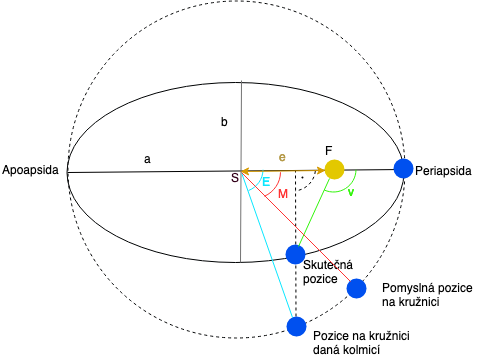
\includegraphics[width=350pt]{Images/Orbit.png}
\caption[Elementy orbity]{Elementy orbity \footnotemark}
\end{center}
\end{figure}

\footnotetext[1]{Vytvořeno autorem v \url{https://www.draw.io}.}

\begin{itemize}
\item \textbf{Anomálie} -- Pokud bychom si orbitu tělesa představili jako kružnici, \textbf{střední anomálie (M)} by byla úhel těleso-střed-periapsida. Tělesa se ale nepohybují po kružnici. Jejich rychlost se v~čase mění a~ohnisko neleží ve středu elipsy. \textbf{Pravá anomálie (v)}~proto označuje úhel těleso-ohnisko-pariapsida. V~případě, že by se těleso nacházelo na pomyslné pozici na kružnici, která by byla určena průsečíkem kružnice a~kolmicí k~hlavní ose elipsy procházející skutečnou pozicí tělesa, \textbf{excentrická anomálie (E)}~by označovala úhel těleso-střed-periapsida.~\cite{kleczek}

\item \textbf{Apoapsida} -- Bod, v~němž se obíhající těleso dostane nejdále od tělesa obíhaného (ohniska). V~případě Země je to 152~097~700~km od Slunce. Specifičtějšími pojmy jsou např. apohelium a~apogeum. To jsou největší vzdálenosti od Slunce a~od Země.~\cite{kleczek}

\item \textbf{Excentricita (e)} -- Výstřednost orbity udává, jak moc je ohnisko vzdáleno od středu orbity. Častěji se ovšem setkáváme s relativní excentricitou, která je rovna poměru absolutní excentricity a~velké poloosy. Kružnice má nulovou výstřednost, elipsa ji má v~intervalu \code{(0,~1)}, útvar s~excentricitou rovnou jedné se nazývá parabola a~výstřednost větší než 1~má hyperbola. Excentricita oběžné dráhy Země je 0,016. Jedná se tak téměř o~kružnici.~\cite{kleczek}

\item \textbf{Keplerovy zákony} -- Jedná se o~3 zákony popisující pohyb planet kolem Slunce. Je možné je aplikovat i~na jiná tělesa pohybující se po eliptické oběžné dráze.~\cite{kleczek}

\begin{enumerate}
\item „Dráha planety je elipsa, v jejímž jednom ohnisku se nachází Slunce.“
\item „Plochy opsané průvodičem planety jsou za stejnou dobu konstantní.“
\item „Druhé mocniny oběžných dob planet jsou ve stejném poměru, jako třetí mocniny velkých poloos.“
\end{enumerate}

\item \textbf{Periapsida} -- Bod, v~němž se obíhající těleso dostane nejblíže tělesu obíhanému (ohnisku). V~případě Země je to 147~098~074~km od Slunce. Specifičtějšími pojmy jsou např. perigalaktikum a~periselenium. To jsou nejmenší vzdálenosti od centra Galaxie a~od Měsíce.~\cite{kleczek}

\item \textbf{Světelný rok (ly)} -- Běžné velikostní jednotky jako kilometry nejsou pro potřeby měření vzdáleností ve vesmíru dostačující. Dokonce i~astronomická jednotka je pro tyto účely příliš malá. Světelný rok je jednotka, jejíž velikost je rovna vzdálenosti, kterou světlo ve vakuu urazí za jeden pozemský rok, což je 9~460~730~472~580~800~m. V~aplikaci jsou používány taktéž kombinace této jednotky a~předpon soustavy SI, např. kly, Mly nebo Gly.~\cite{kleczek}

\item \textbf{Velká poloosa (a)} -- Největší možný poloměr orbity. Jedná se o~aritmetický průměr z~apoapsidy a~periapsidy. V případě Země tato velikost činí 149~597~887~km. Z~této vzdálenosti byla dříve odvozena astronomická jednotka (AU). Definice této jednotky se ale časem vyvíjela a nakonec se ustálila na hodnotě 149~597~870~700~m.~\cite{kleczek}
\end{itemize}

\section{Použité technologie}

\subsection{Jazyk TypeScript}

\textit{TypeScript} je programovací jazyk vyvinutý firmou \textit{Microsoft}. Jedná se o~nádstavbu jazyka \textit{JavaScript}, která přidává statické typování a~další vlastnosti objektového programování. Kód napsaný v~jazyce \textit{JavaScript} je kompatibilní s~\textit{typescriptovým} kódem. Pro kompatibilitu v~prohlížečích je nutné veškerý \textit{TypeScript} transpilovat do \textit{javascriptového} kódu.~\cite{typescript}

\subsection{Knihovna React}

Javascriptová knihovna \textit{React}, jejíž autorem je \textit{Facebook}, usnadňuje a~zefektivňuje tvorbu \textit{UI}.~\cite{reactbook} Přináší tzv. \textit{one-way data binding}, které zaručuje okamžitou aktualizaci \textit{UI} při změně stavu aplikace.~\cite{onewaydatabinding} \textit{React} si vytváří vlastní virtuální \textit{DOM}, který je na rozdíl od toho v~\textit{HTML} rychlejší. V tomto modelu pak React provádí všechny své operace. Teprve když je třeba provést změnu v~prohlížeči, je třeba  aktualizovat \textit{HTML}.~\cite{reactbook}

\subsubsection{Syntaxe TSX}

Vytvářet zanořovací strukturu komponent může být nepřehledné. Proto se často s~knihovnou \textit{React} používá i~syntaxe \textit{JSX}. Ta umožňuje psát \textit{javascriptový} kód v~podobě \textit{XML} tagů. \textit{JSX} syntaxi je z~důvodů kompatibility prohlížečů nutné transpilovat do nativního \textit{JavaScriptu}.~\cite{reactbook} TSX je pak obdoba JSX v~jazyce TypeScript.

\lstinputlisting[caption={Porovnání JS a~JSX}, language={JavaScript}]{SourceCodes/JSX.js}

\subsection{Knihovna Three.js}

\textit{Three.js} je javascriptová knihovna usnadňující práci s~\textit{WebGL}. To je rozhraní, které umožňuje přístup k \textit{HW} komponentám počítače specializovaných pro zpracování grafiky 2D a~3D grafiky přes \textit{JavaScript}. Veškerou tuto grafiku je možno vykreslovat v~prohlížeči za využití elementu \code{canvas}.~\cite{graphic}

\subsection{Framework Node.js}

Framework \textit{Node.js} umožňuje používání jazyka \textit{JavaScript} na serveru. Pracuje pouze s~jediným vláknem a~funguje na asynchronním neblokujícím zpracování požadavků. Jakmile je dokončen požadavek, jeho callback uvedený v argumentu se zařadí do fronty.  Tzv. \textit{event loop} pak zjišťuje, zda je zásobník zpracovávaných operací prázdný. Pokud ano, vloží do něj první callback z~fronty. Tento cyklus se opakuje po celou dobu běhu serveru.~\cite{node}

\subsection{Databáze MongoDB}

\textit{MongoDB} je \textit{NoSQL} multiplatformní dokumentová databáze s~otevřeným zdrojovým kódem. Narozdíl od relačních databází používá dokumenty ve formátu \textit{BSON}, což je binární obdobou \textit{JSON}. Při vytváření dokumentů si databáze automaticky vytváří vlastní unikátní ID.  Uložené dokumenty lze mimo jiné vyhledávat na základě prvků v~poli, podle rozsahu nebo podle regulárních výrazů. V~\textit{MongoDB} je možné indexovat libovolné pole. Indexy jsou koncepčně podobné, jako v~relačních databázích.~\cite{mongomongoose}

\subsection{Knihovna Mongoose}
Knihovna \textit{Mongoose} pro JavaScript zjednodušuje práci s~MongoDB, zejména pak vytváření schémat a~validaci dat. Umožňuje práci s pluginy, což jsou uživatelské funkce, které po zaregistrování na daném schématu mohou zautomatizovaně provádět předem definované činnosti nebo reagovat na různé událost.~\cite{mongomongoose}

\subsection{Nástroj Swagger UI}
\textit{Swagger UI} je nástroj pro vizualizaci specifikace \textit{Open API}. Vygenerovaný interaktivní webový dokument umožňuje vytvářet \textit{HTTP} požadavky na cílové rozhraní a~zobrazit výsledek těchto požadavků.~\cite{swaggerui}

\subsection{Nástroj Webpack}
Prohlížečový \textit{JavaScript} nativně nepodporuje rozdělování kódu do modulů (jako např. \textit{Java} do balíčků nebo \textit{C++} do jmenných prostorů). Jediným způsobem je importovat do \textit{HTML} větší množství \textit{javascriptových} souborů pomocí tagu \code{<script>}. Tento postup je ale špatnou praktikou a~na web má negativní dopady.~\cite{jsconcat}

Díky nástroji \textit{Webpack} je možné v~\textit{JavaScriptu} využívat modulární systémy jako \textit{CommonJS}, \textit{AMD} nebo \textit{ES modules}. Je tak možné větší množství souborů propojit pomocí klauzulí \code{require} nebo \code{import}.~\cite{webpack}

\textit{Webpack} také umožňuje využívat tzv. \textit{loadery} třetích stran. To vede k možnosti podobně načítat, slučovat či parsovat i soubory jiných typů, např. \textit{CSS}, \textit{SVG} nebo \textit{JSON}. Zároveň za využití bohaté nabídky pluginů lze všechny tyto soubory modifikovat, např. převádět nový \textit{JavaScript} verze \textit{ES6} na starší, podporovaný prohlížeči.~\cite{webpack}

\lstinputlisting[caption={Konfigurace nástroje Webpack}, language={JavaScript}]{SourceCodes/Webpack.js}.

\subsection{Verzovací systém Git}

\textit{Git} je systém správy verzí vytvořený \textit{Linusem Torvaldsem}. Při vytváření nové verze dat vytvoří snímky všech souborů tak, jak v daný okamžik vypadají a~na tyto snímky pak uloží reference. V~případě, že se soubor nijak nemění se nevytváří nový snímek, ale pouze se nastaví reference na ten předchozí, který je identitický.~\cite{git}

Pro spravované soubory používá tři stavy. Při změně souboru se nastaví jeho stav na \textit{modified}. Stav \textit{staged} znamená, že soubor byl označen k tomu, aby byl zapsán v další verzi. Zapsaný soubor je ve stavu \textit{commited}. Všechny tyto změny jsou však pouze lokální. Pro umístění změn do vzdáleného repozitáře je třeba všechny zapsané soubory odeslat \textit{(push)}. Ostatní s~přístupem do repozitáře si pak mohou tyto změny stáhnout \textit{(pull)}.~\cite{git}

\subsection{Balíčkovací systém NPM}

\textit{NPM} je správce balíčků pro serverový i~klientský \textit{JavaScript}. Řídícím souborem v projektu je \textit{package.json}, který obsahuje informace o~projektu a~určuje, které balíčky jsou součástí projektu.  Všechny balíčky jsou umístěny do adresáře \textit{node\_modules} v~projektu. Součástí je také soubor \textit{package-lock.json}, který zachovává verze nainstalovaných balíčků.~\cite{nodebook}

\lstinputlisting[caption={Ukázka práce s~NPM}, language={JavaScript}]{SourceCodes/Npm.txt}.

\vspace*{-1.5cm}
\subsection{Preprocesor SASS}

Preprocesor \textit{SASS} přidává do \textit{CSS} možnost zanořování selektorů, proměnné, funkce, podmínky a~další vlastnosti zlepšující čitelnost kódu. Pro kompatibilitu s~prohlížeči je nutné ho transpilovat do \textit{CSS}.~\cite{sass}

\section{Návrh a~vývoj aplikace}

\subsection{Struktura projektu}

React nepřichází s~žádnou doporučenou strukturou projektu.~\cite{filestructure} Proto došlo k~vytvoření vlastní struktury. Vzhledem k~velkému množství souborů je celý obsah projektu členěn do adresářů a~modulů.

\begin{itemize}
\item \textbf{dist}: Produkční sestavení aplikace. Veškerý obsah adresáře se generuje automaticky.
\item \textbf{node\_modules}: Externí knihovny pro serverovou část.
\item \textbf{src}: Zdrojové soubory aplikace.

\begin{itemize}
\item \textbf{Client}: Podprojekt, který obsahuje všechny klientské soubory.

\begin{itemize}
\item \textbf{node\_modules}: Externí knihovny pro klientskou část.
\item \textbf{src}:  Zdrojové soubory klientské části.

\begin{itemize}
\item \textbf{Controls}: Modul obsahující ovladače a~tlačítka využitá v~menu.
\item \textbf{Forms}: Modul umožňující tvorbu formulářů.
\item \textbf{Global}: Hlavičkové soubory dostupné v~globálním prostoru.
\item \textbf{Panel}: Modul pro panel tělesa.
\item \textbf{System}: Hlavní modul obsahující systémové soubory.
\item \textbf{Universe}: Modul zprostředkovávající simulátor.
\item \textbf{User}: Modul s~formuláři a~další komponentami pro uživatele.
\item \textbf{Utils}: Pomocný modul.
\end{itemize} 

\end{itemize} 

\item \textbf{Constants}: Konstanty a~konfigurace.
\item \textbf{Controllers}: Kontrolery s~adresářovou strukturou popisující REST~API.
\item \textbf{Database}: Databázové soubory.

\begin{itemize}
\item \textbf{Plugins}: Databázové pluginy.
\item \textbf{Schemas}: Databázová schémata.
\end{itemize} 

\item \textbf{Global}: Hlavičkové soubory dostupné v~globálním prostoru.
\item \textbf{Models}: Modelové třídy obsahující aplikační logiku.
\item \textbf{Public}: Vstupní HTML soubor a~další statické soubory.

\begin{itemize}
\item \textbf{Fonts}: Písma.
\item \textbf{Images}: Obrázky rozčleněné do podadresářů.
\item \textbf{JavaScript}: Javascriptové soubory.
\end{itemize} 

\item \textbf{Utils}:  Pomocné třídy.
\end{itemize} 

\end{itemize} 

Moduly obsažené zejména v~klientské části projektu jsou adresářové celky, které mohou obsahovat další strukturu:

\begin{itemize}
\item \textbf{Components}: React komponenty.
\item \textbf{Constants}: Konstanty a konfigurace modulu.
\item \textbf{Redux}: Akce a reducer.
\item \textbf{Styles}: Styly.
\item \textbf{Views}: Pohledy.
\end{itemize} 

Každý modul obsahuje mapování a~export všech souborů, které mají být veřejné. Z~vnějšku není nutné znát strukturu daného modulu a~adresu hledaného souboru uvnitř modulu.


\lstinputlisting[caption={Správné a~nesprávné použití importu souboru z~modulu}, language={JavaScript}]{SourceCodes/ImportFromModule.js}


\subsection{Uživatelské rozhraní}

Klientská část aplikace dodržuje architekturu \textit{Redux}. Všechen stav aplikace je na jednom místě v~tzv. \textit{store}, odkud ho mohou číst všechny komponenty, jež jsou na \textit{store} napojené. Kdykoliv se změní stav aplikace, dojde k~automatickému překreslení těch částí \textit{UI}, které změněná data obsahují.~\cite{reactbook}

Stav aplikace lze změnit zavoláním funkce \textit{dispatch}, jejímž argumentem bude právě prováděná akce. Akce je prostým objektem, který obsahuje povinnou vlastnost \code{type} s~typem akce a~libovolné další vlastnosti. Jelikož akce by měly být znovupoužitelné, jsou často umístěny v~\textit{action creator}. To je funkce, která akci vrací.~\cite{reactbook}

\begin{figure}[H]
\begin{center}
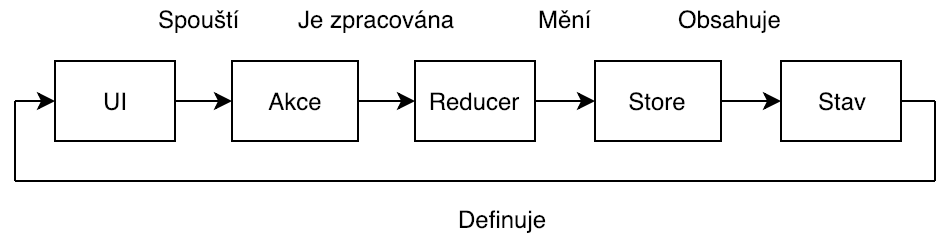
\includegraphics[width=350pt]{Images/Redux.png}
\caption[Životní cyklus architektury Redux]{Životní cyklus architektury Redux \footnotemark}
\end{center}
\end{figure}

\footnotetext[1]{Vytvořeno autorem v \url{https://www.draw.io}.}

Samotná změna stavu je pak provedena ve funkci \textit{reducer}. Ten ze starého stavu aplikace a~akce vytvoří a~vrátí nový stav.  Obsahem \textit{reduceru} je často rozsáhlý \textit{switch} s~výčtem všech akcí, kde je u~každé akce uvedena její modifikace stavu. Aby změna stavu aktualizovala všechny komponenty, které tomuto stavu naslouchají, je nutné, aby \textit{reducer} vracel vždy nově vytvořený objekt, nikoliv pouze pozměněný ten starý.~\cite{reactbook}

\lstinputlisting[caption={Ukázka architektury Redux}, language={JavaScript}]{SourceCodes/Redux.js}

\subsubsection{Akce}

Vytvářet zejména asynchronní akce manuálně je zdlouhavé. Pro správnou funkcionalitu \textit{UI} je totiž při asynchronním požadavku třeba zaznamenat následující stavy:

\begin{itemize}
\item \textbf{SENT}: Požadavek byl odeslán,
\item \textbf{SUCCESS}: Požadavek byl úspěšně ukončen,
\item \textbf{FAIL}: Požadavek byl neúspěšně ukončen.
\end{itemize}

V~projektu byla proto vytvořena vlastní knihovna \textit{Redux} v~modulu \textit{Utils}, která zajišťuje vykonávání několika typů akcí:

\begin{itemize}
\item \textbf{setAction}: Nastavení hodnoty,
\item \textbf{toggleAction}: Přepnutí hodnoty (generuje \textit{ON/OFF}),
\item \textbf{asyncAction}: Asynchronní požadavek (generuje \textit{SENT/SUCCESS/FAIL}).
\end{itemize}

V~kódu pak použití asynchronní akce vypadá následovně. Automaticky je zajištěno sledování průběhu požadavku a~je tudíž je jednoduše možné zobrazit např. načítací animaci.

\lstinputlisting[caption={Redux akce za využití vlastní knihovny}, language={JavaScript}]{SourceCodes/ReduxAction.js}

\subsubsection{Reducer}

Reducer je běžně funkce, která obsahuje \textit{switch} s~výčtem všech akcí a~jejich modifikací stavu aplikace.~\cite{reactbook} Díky vlastní knihovně to ale není nutné. Stačí uvést pole všech akcí a~případně i~počáteční stav \textit{store}.

\lstinputlisting[caption={Redux reducer za využití vlastní knihovny}, language={JavaScript}]{SourceCodes/ReduxReducer.js}

\subsection{3D grafika}

Před vykreslováním těles ve vesmíru je nutné ze serveru nejdříve získat data k~těmto tělesům. Následovně je použita třída \textit{BodyFactory}, která z~datových objektů těles vytvoří kontejnery obsahující kromě samotných dat z~databáze také objekty pro vykreslení popsané v~podkapitolách této kapitoly.

Celý vesmír je neustále v~pohybu. Měsíc obíhá planetu Zemi, která se pohybuje kolem Slunce. Slunce i~s~celou soustavou obíhá střed naší galaxie. Mléčná dráha se pak volně pohybuje v~rámci místní kupy galaxií a~ta zas v~rámci místní nadkupy galaxií. \cite{kleczek}  Počítat absolutní pozici tělesa by proto bylo více než náročné.

Je proto důležité, aby každé těleso bylo umístěno mezi potomky tělesa, kolem kterého zdánlivě obíhá. Tím je dosaženo dědičnosti a~souřadnice není nutné uvádět absolutně vzhledem k~vesmíru, ale pouze vzhledem k~rodičovskému tělesu. Pro práci s~3D grafikou byla v~rámci projektu vytvořena vlastní třída \textit{Scene}. Ta v~každém průběhu vykreslovací smyčky vypočítá pozice a~rotace těles a~aktualizuje je.

\lstinputlisting[caption={Práce s vlastní knihovnou pro 3D grafiku}, language={JavaScript}]{SourceCodes/Scene.js}

\subsubsection{Těleso}

Samotné těleso je reprezentováno koulí, tedy objektem s~geometrií \textit{THREE.SphereGeometry}. Pokud má těleso rozdílný rovníkový a~polární průměr, je výsledné zploštění řešeno transformaci \textit{new THREE.Matrix4().makeScale()}. Materiálem je \textit{THREE.MeshBasicMaterial} (tělesa emitující světlo) nebo \textit{THREE.MeshPhongMaterial} (tělesa pohlcující světlo). Povrch tělesa tvoří 2D~textura \textit{THREE.Texture} tvořená obrázkem ve formátu \textit{JPG}.

\begin{figure}[H]
\begin{center}
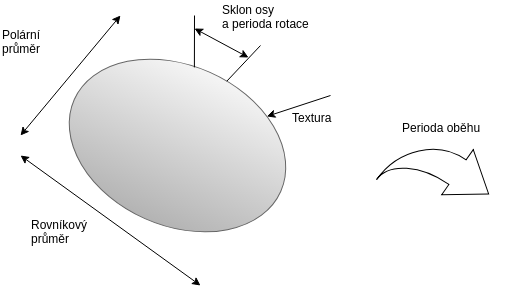
\includegraphics[width=370pt]{Images/BodyData.png}
\caption[Jednoznačná definice tělesa]{Jednoznačná definice tělesa \footnotemark[1]}
\end{center}
\end{figure}

\footnotetext[1]{Vytvořeno autorem v \url{https://www.draw.io}.}

\subsubsection{Orbita}

Orbita je objekt s geometrií \textit{THREE.Geometry}, jejíž eliptický tvar je vypočten na základě nejmenší (periapsida) a~největší (apoapsida) vzdálenosti tělesa od těžiště  a~výstřednosti dráhy (excentricita).~\cite{kleczek} Jako materiál je použit \textit{THREE.LineMaterial}.

\lstinputlisting[caption={Výpočet geometrie orbity tělesa}, language={JavaScript}]{SourceCodes/Orbit.js}


\begin{figure}[H]
\begin{center}
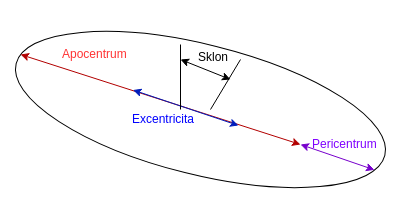
\includegraphics[width=320pt]{Images/OrbitData.png}
\caption[Jednoznačná definice orbity tělesa]{Jednoznačná definice orbity tělesa \footnotemark[1]}
\end{center}
\end{figure}

\vspace*{-1cm}
\subsubsection{Světlo}

Pokud je těleso zdrojem viditelného světla, je mezi jeho potomky navíc také bodové světlo\newline \textit{THREE.PointLight}, které emituje světlo o~stejné barvě a~intenzitě, jakou má reálné těleso.

\subsubsection{Prstence}

Prstenec je objekt s~geometrií \textit{THREE.BufferRingGeometry}, materiálem\newline \textit{THREE.MeshLambertMaterial} a~\textit{2D}~texturou \textit{THREE.Texture} tvořenou obrázkem ve formátu \textit{JPG} nebo \textit{PNG}. Těleso může mít libovolný počet prstenců, nebo také žádný.

\begin{figure}[H]
\begin{center}
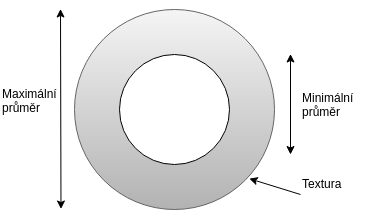
\includegraphics[width=280pt]{Images/RingData.png}
\caption[Jednoznačná definice prstence tělesa]{Jednoznačná definice prstence tělesa \footnotemark[1]}
\end{center}
\end{figure}

\footnotetext[1]{Vytvořeno autorem v \url{https://www.draw.io}.}

\subsubsection{Popisek}

Popisek je reprezentován \textit{HTML} elementem, který je absolutně pozicován na stejné souřadnice, jako je vykreslované těleso. Kromě názvu tělesa obsahuje i~aktuální rychlost pohybu, vzdálenost od Země, vzdálenost od kamery a~vzdálenost od centrálního tělesa.

\subsubsection{Částice}
Protože aplikace obsahuje řádově pouze desítky až stovky těles, je nemožné zobrazit rozsáhlejší struktury, které jsou jinak typické pro danou oblast ve vesmíru. Příkladem může být \textit{Kuiperův pás} nebo \textit{Oortův oblak} v~naší sluneční soustavě. Tato uskupení obsahují stovky miliard planetek, komet nebo~dalších těles. \cite{kleczek}

Pro tyto účely se v aplikaci využívá pseudonáhodné generování částic pomocí\break\textit{THREE.Points}. V~závislosti na typu tělesa (pás, oblak, hvězdokupa, ...) je využito pro rozmístění částic buď rovnoměrné, normální nebo exponenciální rozdělení.  Protože zde ale figuruje náhoda, nemusí takto vygenerovaná tělesa odpovídat realitě a~jedná se pouze o~vizuální doplnění prázdného prostoru. Uživatel může zobrazení částic kdykoliv vypnout.

\begin{figure}[H]
\begin{center}
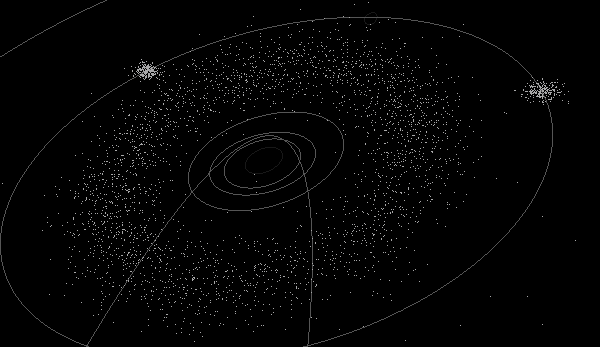
\includegraphics[width=450pt]{Images/Particles.png}
\caption{Hlavní pás planetek vygenerovaný pomocí částic}
\end{center}
\end{figure}

Funkce pro generování částic je uložena v~databázové kolekci typů těles jako textový řetězec. Je možné tak vytvořit jedinou funkci, např. pro generování spirálních galaxií, a~z~tohoto typu pak vytvářet instance těles o~stejném tvaru, lišících se v ostatních fyzikálních vlastnostech. Protože ale administrátor vše musí nejdříve schválit, je tím zároveň ošetřena bezpečnostní hrozba, kdy by uživatel do generující funkce umístil škodlivý kód.

\lstinputlisting[caption={Naplnění geometrie částicemi ve tvaru koule}, language={JavaScript}]{SourceCodes/Particles.js}

\vspace*{-0.6cm}
\subsection{Pohyb těles}

Na aplikaci lze pohlížet jako na simulátor, protože výpočet vzájemné pozice těles v~čase nelze vypočítat pouhým vyjádřením neznámé z~rovnice a~je nutno podstoupit proces, který k~výsledku postupně povede. Na druhou stranu, aplikace se řídí podle Keplerových zákonů. Ty říkají, jak se tělesa pohybují, ale neříkají proč.~\cite{kleczek} Nepracuje se se skutečnými fyzikálními vztahy, pouze s~pravidly která vychází z~Keplerových zákonů. Z~tohoto pohledu by se tak jednalo spíše o~emulátor.

\subsubsection{Výpočet konstatních dat}

Při načtení tělesa z databáze jsou vypočítány hodnoty, které jsou pro dané těleso konstantní. Pro úplnost jsou zde uvedeny i~výpočty, které přímo nesouvisí s~pohybem tělesa. O~jejich dopočítání se stará plugin zaregistrovaný na schématu těles. Jako první jsou u~každého tělesa dopočítány \textbf{poloosy orbity} a~\textbf{gravitační parametr}:

\vspace*{-0.5cm}
$$a = \frac{d_{max} - d_{min}}{2}~~~~~~~~~~b = a - \sqrt{1 - e^2}~~~~~~~~~~\mu = M * G$$
\begin{center}
\textit{a -- hlavní poloosa, b -- vedlejší poloosa, $d_{max}$ -- apoapsida, $d_{min}$ -- periapsida, e~--~excentricita, $\mu$ -- gravitační parametr, M -- hmotnost tělesa}~\cite{kleczek}
\end{center}

Výpočet \textbf{obvodu} a~\textbf{obsahu orbity} a~\textbf{oběžné doby}:

\vspace*{-0.5cm}
$$O \approx \pi * \sqrt{2 * (a^2 + b^2)}~~~~~~~~~~S = \pi * a * b~~~~~~~~~~T = 2 * \pi * \sqrt{\frac{a^3}{\mu}}$$
\begin{center}
\textit{O -- obvod orbity, S -- obsah orbity, a -- hlavní poloosa, b -- vedlejší poloosa, T -- oběžná doba, $\mu$ -- gravitační parametr}~\cite{kleczek}
\end{center}

Výpočet \textbf{rovníkového obvodu}, \textbf{objemu} a~odhadovaného \textbf{povrchu tělesa}:

\vspace*{-0.5cm}
$$O \approx \pi * \sqrt{2 * (r_{x}^2 + r_{z}^2)}~~~~~~~~~~V \doteq \frac{4}{3} * \pi * r_{x} * r_{y} * r_{z}~~~~~~~~~~S \doteq 4 * \pi * r_{x} * r_{y}$$
\begin{center}
\textit{V -- objem tělesa, r -- poloměr tělesa, O -- rovníkový obvod tělesa, S -- povrch tělesa}~\cite{kleczek}
\end{center}

Výpočet \textbf{hustoty}, \textbf{zploštění} a~\textbf{maximální} nebo \textbf{minimální orbitální rychlosti}:

\vspace*{-0.5cm}
$$\varrho = \frac{M}{V}~~~~~~~~~~f = 1 - \frac{r_{y}}{r_{x}}~~~~~~~~~~v_{max} = \sqrt{\mu * \frac{2}{d_{min}} - \frac{1}{a}}$$
\begin{center}
\textit{$\varrho$ -- hustota, M -- hmotnost tělesa, V -- objem tělesa, f~--~zploštění tělesa, r -- poloměr tělesa, $v_{max}$ -- max. rychlost, $\mu$ -- gravitační parametr, $d_{min}$, periapsida}~\cite{kleczek}
\end{center}

Výpočet \textbf{gravitačního zrychlení}, \textbf{únikové rychlosti} a~popř. i~\textbf{svítivosti}:

\vspace*{-0.5cm}
$$a = G * M * r^2~~~~~~~~~~v = \sqrt{\frac{2 * \mu}{r}}~~~~~~~~~~L = 4 * \pi * r^2 * \sigma * T^4$$
\begin{center}
\textit{a -- gravitační zrychlení, M -- hmotnost, r -- poloměr, v -- úniková rychlost, $\mu$ -- gravitační parametr, L -- svítivost, $\sigma$ -- Stefan-Boltzmannova konstanta, T -- povrchová teplota}~\cite{kleczek}
\end{center}

Výpočet \textbf{rovníkové rychlosti} a~\textbf{úhlové rychlosti} rotace:

\vspace*{-0.5cm}
$$v = \frac{O}{T}~~~~~~~~~~\omega = \frac{2 * \pi}{T}$$
\begin{center}
\textit{v -- rychlost rotace, O -- rovníkový obvod, T -- perioda rotace, $\omega$ -- úhlová rychlost}~\cite{kleczek}
\end{center}


\subsubsection{Inicializace pozice}

Při načtení scény je nutno inicializovat pozici všech těles. V~databázi je u~každého tělesa uložený datum, v~němž těleso prošlo periapsidou. Následně dojde k~výpočtu rozdílu dnešního data a~data průchodu periapsidou. Dále dojde k výpočtu excentrické anomálie E~--~úhlu, jenž svírá spojnice periapsidy se středem orbity a~spojnice pozice tělesa na pomyslné kruhové orbitě se středem orbity. Toho lze docílit pomocí Keplerovy rovnice.~\cite{kleczek}

\vspace*{-0.5cm}
$$E -  \epsilon * sin(E) = \frac{2 * \pi}{T} * ((t - t\textsubscript{0})~mod~T)$$
\begin{center}
\textit{E -- excentrická anomálie, $\epsilon$ -- absolutní excentricita, T -- perioda oběhu, t -- aktuální čas, t\textsubscript{0} -- čas v~pericentru}~\cite{kleczek}
\end{center}

\begin{figure}[H]
\begin{center}
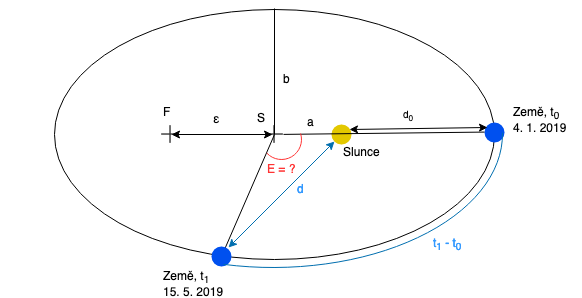
\includegraphics[width=350pt]{Images/Initial.png}
\caption[Výpočet výchozí pozice tělesa]{Výpočet výchozí pozice tělesa (poměry velikostí nejsou realistické) \footnotemark[1]}
\end{center}
\end{figure}

\footnotetext[1]{Vytvořeno autorem v \url{https://www.draw.io}.}

\vspace*{-0.5cm}
Vyjádření excentrické anomálie E~z~Keplerovy rovnice není možné. Pro přibližný výpočet byla proto zvolena Newtonova iterační metoda, pomocí níž se výsledek jednotlivými kroky stále zpřesňuje, až dokud přesnost nedosáhne požadované hranice přesnosti, což je v tomto případě miliontina radiánu.

\vspace*{-0.5cm}
$$E\textsubscript{n} = \frac{2 * \pi}{T} + \epsilon * sin(E\textsubscript{n - 1})$$
\begin{center}
\textit{E\textsubscript{n} -- excentrická anomálie n-té iterace, $\epsilon$ -- absolutní excentricita, T -- perioda oběhu}~\cite{michalrepik}
\end{center}

Z~E~je možné získat \textbf{skutečnou anomálii} \textit{v}:

\vspace*{-0.5cm}
$$v = 2 * arctg\Bigg(\sqrt{\frac{1 + e}{1 - e}} * tg\bigg(\frac{E}{2}\bigg)\Bigg)$$
\begin{center}
\textit{v -- skutečná anomálie, E -- excentrická anomálie, e -- excentricita}~\cite{michalrepik}
\end{center}

Dále je třeba \textbf{úhel mezi spojnicemi střed-periapsida a~střed-těleso}. To je problém trojúhelníku střed-Slunce-Země, na který se aplikuje kosinová věta.

\vspace*{-0.5cm}
%$$|SZ| = \sqrt{\epsilon^2 + d^2 * 2 * \epsilon * d * cos(\pi - v)}$$
$$\varphi = arccos\Bigg(\frac{d^2 - \epsilon^2 - d\textsubscript{s}^2}{2 * \epsilon * d\textsubscript{s}}\Bigg)$$
\begin{center}
\textit{d -- |Země-těžiště|, d\textsubscript{s} -- |Země-střed|, $\epsilon$ -- absolutní excentricita}~\cite{michalrepik}
\end{center}

Knihovna THREE.js umožňuje získat souřadnice bodu na elipse podle zadaného úhlu. Těleso tak může být umístěno do výchozí pozice odpovídající úhlu $\varphi$ v~rámci jeho orbity.

\subsubsection{Inicializace rotace}

U inicializace rotace se počítá s~tím, že rychlost rotace tělesa je na rovníku konstantní. V~databázi je uložen datum, v němž mělo těleso nulový úhel rotace v~rámci dané souřadnicové soustavy. Následně dojde k~výpočtu úhlu, o~něhož se stihlo za tento rozdíl časů těleso pootočit kolem své osy.

\vspace*{-0.5cm}
$$\varphi = 2 * \pi * \frac{(t - t\textsubscript{0})~mod~T}{T}$$

\begin{center}
\textit{$\varphi$ -- úhel rotace, T -- perioda oběhu, t -- aktuální čas, t\textsubscript{0}~--~výchozí čas}
\end{center}

\subsubsection{Vykreslovací smyčka}

Jakmile jsou pozice a~rotace těles inicializovány, je třeba je s~ubíhajícím časem aktualizovat. Nejdříve je nutné zjistit, \textbf{kolik milisekund uplynulo} od posledního vykreslení a~podle toho i~aktualizovat čas simulátoru.

\begin{center}
$\Delta t = t - t_{0}~~~~~~~~~~t_{s} = t_{s} + \Delta t * k$

\textit{$\Delta t$ -- čas od posledního vykreslení, t -- aktuální čas, t\textsubscript{0} -- čas posledního vykreslení, $t_{s}$~--~čas simulátoru, k~--~rychlost běhu času}
\end{center}

Nová \textbf{pozice tělesa} je určena opětovným vyřešením Keplerovy rovnice. Počet iterací pro dosažení požadované přesnosti roste společně s~excentricitou orbity. Avšak i~u~dlouhoperiodických komet, jejichž excentricita dosahuje často i~0,999 lze najít dostatečně přesnou excentrickou anomálii do 5 iterací. Je tak dosaženo dobré přesnosti za cenu malého snížení výkonu. Pokud by nová pozice byla vypočítána ze staré pozice, ke které by se pouze přičetla uražená dráha, jednotlivé nepřesnosti by se postupně sčítaly a~bylo by nutné je kompenzovat. 

Jiná situace nastává u~aktualizace \textbf{rotace tělesa} kolem osy, jejíž rychlost se v~čase nemění. Ta je uskutečněna jednoduchým přičtením úhlu, o~nějž se těleso otočí za dobu, která uplynula od posledního vykreslení, k~aktuálnímu úhlu.

\vspace*{-0.5cm}
$$\varphi = \varphi + \omega * \Delta t$$
\begin{center}
\textit{$\varphi$ -- úhel rotace, $\omega$ -- úhlová rychlost rotace, $\Delta t$ -- čas od posledního vykreslení}
\end{center}

Dále dojde k výpočtu údajů pro popisky. \textbf{Vzdálenost tělesa od ohniska} určí knihovní metoda v~THREE.js \code{bodyPosition.distanceTo(parentPosition)}. Stejným způsobem dojde k~určení \textbf{vzdálenosti tělesa od Země a~od kamery}. Následně je vypočítána \textbf{okamžitá rychlost tělesa}.

\vspace*{-0.5cm}
$$v = \sqrt{\mu * \frac{2}{d} - \frac{1}{a}}$$
\begin{center}
\textit{v -- okamžitá rychlost, $\mu$ -- gravitační parametr, d -- vzdálenost od ohniska}~\cite{kleczek}
\end{center}

Nakonec jsou aktualizovány samotné popisky. Výše zmíněné údaje se počítají samozřejmě pouze pokud je zobrazení popisku s~danou informací aktivováno.

\subsubsection{Omezení}

Aplikace zanedbává některé z~aspektů, které v~realitě existují. Důvodem může být vysoká výpočetní náročnost pro prohlížeč nebo složitost implementace. V~důsledku toho může v~simulátoru docházet k~nepřesnostem nebo omezeným možnostem vykreslování těles.

\begin{itemize}
\item Hmotnost obíhajících těles je zanedbána. Centrální těleso tak není ovlivněno tělesy obíhajícími. Oběh je počítán na základě Keplerových zákonů a~není třeba řešit vzájemné gravitační ovlivňování těles. V případě vícehvězdných systémů, u~kterých je nezanedbatelná hmotnost více těles, je možné vytvořit virtuální těleso, které se nebude zobrazovat a~které představuje těžiště soustavy, kolem něhož budou ostatní tělesa obíhat.

\item Tělesa s~neperiodickou nebo neeliptickou oběžnou dráhou mají pevně nastavenou pozici a~nepohybují se.

\item Periapsida se vždy nachází přímo na opačné straně elipsy, než apoapsida. Pokud je oběžná dráha příliš excentrická, může se pozice skutečně nejbližšího bodu k~těžišti dráhy a~periapsidy v~aplikaci lišit.

\item Jsou zanedbány dlouhodobé události, např. postupné vzdalování Měsíce od Země o~38~mm za rok.~\cite{rees}
\end{itemize}

\subsection{Serverová část}

\subsubsection{Zachycení HTTP požadavku}

Server vystavuje \textit{REST~API}~\cite{nodebook}, ze kterého si mohou klientské aplikace (v~tomto případě pouze webová aplikace) stahovat data. Rozhraní má jasně danou strukturu a~jeho implementace a~dokumentace je provedena pomocí nástroje \textit{Swagger}. Ten umožňuje sestavit rozhraní z~fyzických souborů. Cesta k~souboru značí adresu \textit{URI} a~obsah zas dostupné metody.

\lstinputlisting[caption={Definice cesty v REST~API}, language={JavaScript}]{SourceCodes/Route.js}

Dokumentace je zpřístupněna na lokální adrese \textit{/api-docs}. Je možné se zde informovat o~všech možných \textit{HTTP} požadavcích nebo je s~nastavenými parametry simulovat.

\subsubsection{Zpracování HTTP požadavku}

Jakmile je přijat požadavek od klienta, musí dojít k následujícím krokům:

\begin{itemize}
\item Zjištění identity uživatele z~tokenu v~hlavičce,
\item Zkontrolování vyžadovaných oprávnění,
\item Obsluha požadavku (načtení a zpracování dat z~DB, ...),
\item Nastavení HTTP statusu, popř. chybového kódu,
\item Odeslání odpovědi.
\end{itemize}

V~aplikaci byla vyvinuta vlastní knihovna, která všechny ze zmíněných procesů automatizuje. Pro většinu druhů zdrojů stačí dva druhy přístupových bodů:

\begin{itemize}
\item Pro všechny zdroje,

\begin{itemize}
\item \textbf{GET}: Vrátí pole zdrojů,
\item \textbf{POST}: Vytvoří nový zdroj a~vrátí zprávu o úspěchu nebo chybě,
\item \textbf{DELETE}: Smaže všechny zdroje a~vrátí počet smazaných zdrojů,
\end{itemize}

\item Pro jeden zdroj,

\begin{itemize}
\item \textbf{GET}: Vrátí jeden zdroj podle ID nebo zprávu o~chybě,
\item \textbf{PUT}: Upraví jeden zdroj podle ID a~vrátí zprávu o~úspěchu nebo chybě,
\item \textbf{DELETE}: Smaže jeden zdroj podle ID a vrátí zprávu o úspěchu nebo chybě.
\end{itemize}

\end{itemize}

Samotná definice přístupových bodů pak může vypadat následovně. U~každé přístupové metody je možné určit, jaká oprávnění musí mít uživatel, aby tuto metodu nad daným zdrojem mohl vykonat.

\lstinputlisting[caption={Zpracování HTTP požadavku}, language={JavaScript}]{SourceCodes/RouteUtils.js}

Modelové třídy většiny entit není nutné psát individuálně. Všechny mají za úkol poskytnout \textit{CRUD operace} nad danou entitou (např. \textit{BodyModel} nad tělesy), případně generovat notifikace či umožnit práci se schvalovacím procesem. Jediné, co se liší, je název databázové kolekce, vybrané sloupce při výpisu detailu entity a~při výpisu všech entit, popř. další parametry. Veškerá logika komunikace s~databází byla ukryta do třídy \textit{ItemModel}. Většina dalších modelů je pak pouhou instancí této třídy s~konkrétními parametry. \textit{ItemModel} vedle \textit{CRUD} operací automatizuje i vytváření notifikací a~schvalovací proces administrátora.

\lstinputlisting[caption={Automatizovaná tvorba modelových tříd}, language={JavaScript}]{SourceCodes/Model.js}

\vspace*{-0.5cm}
\subsection{Databáze}

Data v~aplikaci se ukládají do databáze \textit{MongoDB} za využití knihovny \textit{Mongoose}. Serverová část se řídí architekturou \textit{MVC} a~k~databázi mají přístup pouze modelové třídy. Struktura databáze je zobrazena v~příloze A na konci tohoto dokumentu.

\subsubsection{Připojení do databáze}

Připojení do databáze je jednoznačně inicializováno textovým řetězcem obsahujícím adresu serveru, název databáze a~v~případě autentifikovaného přístupu i~jméno a~heslo uživatele, adresu serveru, port a~název databáze. Dále je třeba zaregistrovat všechna schémata, která budou v~aplikaci využita. Pokud kolekce s nově zaregistrovaným schématem neexistuje, dojde k jejímu automatickmu vytvoření. Je také možné reagovat na úspěšné připojení nebo na chybu.~\cite{nodebook}

Veškerou tuto funkcionalitu obstarává třída \textit{Database}, která byla vytvořena v~rámci projektu. Instance této třídy je staticky (pouze jednou, při spuštění serveru~\cite{nodebook}) vytvořena ve třídě \textit{Model}, který je předkem všech ostatních modelových tříd. Třída \textit{Model} pak tuto instanci databáze poskytuje jako instanční proměnnou s~modifikátorem přístupu \code{protected} všem svým potomkům.

\lstinputlisting[caption={Připojení k databázi v~aplikaci}, language={JavaScript}]{SourceCodes/DatabaseConnection.js}

\vspace*{-0.5cm}
\subsubsection{Mongoose schéma}

Pomocí schématu lze určit strukturu databázové kolekce a~nastavit validační pravidla. Veškerá konfigurace je umístěna v~objektu, který se dosadí jako parametr při vytváření nové instance schématu. Je možné také vytvořit např. indexy přes více polí.~\cite{nodebook}

\lstinputlisting[caption={Vytvoření databázového schématu}, language={JavaScript}]{SourceCodes/Schema.js}

\vspace*{-0.5cm}
\subsubsection{Mongoose plugin}

Pokud je třeba reagovat na jednotlivé události v kolekci (smazání, vložení, ...), lze toho docílit pomocí pluginů. To jsou obdoby spouští z relačních databází. Jedná se o~uživatelem definované funkce, jež dostanou v~parametru schéma, na kterém jsou zaregistrovány. Na tomto schématu pak mohou definovat operace \code{pre} nebo \code{post} s~jednotlivými událostmi a~jejich obsloužení.~\cite{nodebook}

\lstinputlisting[caption={Vytvoření a~použití databázového pluginu}, language={JavaScript}]{SourceCodes/Hash.js}

Ve zdrojovém kódu výše je zobrazena část pluginu pro automatické hashování hesla. Ten při každé změně daného pole nový obsah zahashuje a~teprve onen hash uloží do databáze namísto původní hodnoty. Protože ale není vyloučené, že bude někdy třeba tento plugin použít také v~jiném schématu a~na jiném poli, plugin byl vytvořen univerzálně. Jméno pole je proto určeno parametrem v~pluginu.

Dalším pluginem v~aplikaci je \textit{FillBodyPlugin}. Aplikace se snaží o~největší možnou automatizaci a~je žádoucí, aby se do databáze ukládala pouze nejnutnější data. Ostatní data jsou automaticky dopočítána z~těch v~databázi. Dopočítaná data jsou popsána v~kapitole 3.4 -- Pohyb tělesa.

\subsubsection{Základní práce s databází}

Databáze umožňuje provádět velké množství operací nad daty v~ní uloženými. Je možné vyhledávat podle konkrétní hodnoty, pole hodnot, regulárních výrazů nebo číselného rozsahu. Takto vyfiltrovaná data lze číst, smazat či editovat. Je také možné nastavit velké množství parametrů, např. maximální počet dokumentů (\textit{limit}), které vyhovují filtru. Mimo jiné je možné také provádět více dotazů do databáze jako atomické operace pomocí transakcí.~\cite{nodebook}

\lstinputlisting[caption={CRUD operace nad kolekcí uživatelů}, language={JavaScript}]{SourceCodes/Database.js}

\vspace*{-0.5cm}
\subsubsection{Aggregation Framework}

V případě složitějších databázových dotazů, na které nestačí předpřipravené metody knihovny \textit{Mongoose}, je možno využít metodu \code{aggregate}, jež umožňuje pracovat s~\textit{Aggregation Frameworkem} databáze \textit{MongoDB}. Ten mimo jiné umožňuje v~tzv. \textit{pipeline} dosadit sekvenci dotazů, které se nad daty postupně provedou. Je tak možné používat např. \code{\$match} (vyhledávání), \code {\$group} (seskupování) nebo \code{\$lookup} (spojování více kolekcí).~\cite{aggregation}

V~aplikaci je tento způsob dotazování použit např. v~\code{[GET] /bodies/{bodyId}}, kdy je třeba z~databáze kromě tělesa na základě jeho ID vybrat z jiných kolekcí i typ tělesa, události v~historii tělesa, diskuse o~tělese, komentáře k~diskusím a~nakonec i~uživatele a~hlasy patřící k~jednotlivým diskusím a~komentářům. Konkrétní podoba dotazu použitého v~aplikaci je zobrazena v~příloze~B~na konci tohoto dokumentu.

I přes skutečnost, \textit{že MongoDB} jakožto dokumentová databáze umožňuje zanořování struktur do sebe~\cite{mongomongoose}, pro jednodušší práci byly pro tělesa, události, komentáře a hlasy vytvořeny samostatné kolekce.

\subsection{Instalace a~spuštění aplikace}

Aplikace je k~dispozici online na adrese \url{https://universis.herokuapp.com}, dokumentace \textit{REST API} pak na \url{https://universis.herokuapp.com/api-docs}.

V~případě instalace na lokální počítač bude třeba stáhnout a~nainstalovat server\textit{Node.js}, balíčkovací systém \textit{NPM} a~databázi \textit{MongoDB}. První dva lze společně stáhnout z~oficiálních stránek \url{https://nodejs.org}, databázi pak z~\url{https://docs.mongodb.com/manual/administration/install-community}.

Pokud přísup do databáze vyžaduje autentifikaci, je třeba v~aplikaci v~souboru\break\code{/src/Constants/Config.ts} vyplnit položky \code{database.username} a~\code{database.password}. Následně může dojít ke zvolení umístění vytvořené databáze a~ke spuštění databázového démona z~terminálu. Cesta k~\code{mongod} se může lišit v~případě jiné verze databáze nebo zvolení jiného umístění při instalaci.

\lstinputlisting[caption={Příkaz pro spuštění databáze}, language={JavaScript}]{SourceCodes/StartDB.js}

Dále je třeba z~terminálu v~kořenovém adresáři tohoto projektu spustit~skript, který do databáze vloží základní data -- několik těles a~především uživatele s~administrátorskými právy (email: \textit{universis.root@gmail.com}, heslo: \textit{aDM!n7paSsw0RD}).

\lstinputlisting[caption={Příkaz pro vložení inicializačních dat do databáze}, language={JavaScript}]{SourceCodes/InsertScript.js}

Pro zprovoznění odesílání emailů (např. uživatelům při registraci), je třeba ve stejném konfiguračním souboru nastavit položky \code{email.sender} a~\code{email.password}.

Následně musí dojít ke~stažení externích balíčků \textit{NPM} pro server i~pro klienta, transpilaci zdrojových kódů do nativního \textit{JavaScriptu} a~spuštění serveru. Pro všechny tyto kroky je v~aplikaci předpřipraven skript pro unixové systémy (testováno na \textit{Ubuntu~18}, \textit{Debian~9} a~\textit{macOS Mojave}) a~pro Windows 10.

\lstinputlisting[caption={Příkaz pro sestavení a~spuštění aplikace}, language={JavaScript}]{SourceCodes/Installation.js}

Po krátké chvíli bude aplikace dostupná na adrese \url{http://localhost:3000}, resp. \url{http://localhost:3000/api-docs}.

\section{Rozvržení aplikace}

\subsection{Hlavní stránka}

Hlavní stránka aplikace obsahuje pouze nezbytné odkazy do dalších částí aplikace. Nepřihlášený vidí odkazy do simulátoru a~přihlašovací stránku. Přihlášený uživatel vidí taktéž odkaz do simulátoru, ale druhé tlačítko slouží pro odhlášení.

\begin{figure}[H]
\begin{center}

\includegraphics[width=450pt]{Images/MainPage.png}
\caption{Hlavní stránka}
\end{center}
\end{figure}

\subsection{Autentifikace uživatele}

\subsubsection{Identita}

Každý uživatel, jenž se chce přihlásit nebo se zaregistrovat, se dostane na stránku, kde musí prokázat svou identitu zadáním emailu. V~závislosti na tom, zda zadaný email již v~databázi existuje bude odkázán na stránku pro přihlášení nebo pro registraci.

\begin{figure}[H]
\begin{center}

\includegraphics[width=250pt]{Images/Identity.png}
\caption{Formulář pro zjištění identity uživatele}
\label{Identity}
\end{center}
\end{figure}

\vspace*{-0.5cm}
\subsubsection{Přihlášení}

Stránka obsahuje formulář pro zadání hesla. Nachází se zde odkaz zpět a~odkaz pro obnovení hesla.

\begin{figure}[H]
\begin{center}
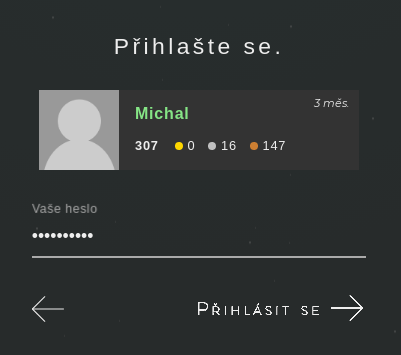
\includegraphics[width=250pt]{Images/SignIn.png}
\caption{Formulář pro přihlášení uživatele}
\label{SignIn}
\end{center}
\end{figure}

\vspace*{-0.5cm}
\subsubsection{Registrace}

Stránka pro zadání a potvrzení hesla k nově vytvářenému účtu. V~případě, že uživatel chce změnit registrační email, je možné se vrátit na stránku se zadáváním identity.

\begin{figure}[H]
\begin{center}

\includegraphics[width=250pt]{Images/SignUp.png}
\caption{Formulář pro registraci uživatele}
\label{SignUp}
\end{center}
\end{figure}

\subsubsection{Zapomenuté heslo}

Na této stránce se nachází formulář s~polem pro email. Po úspěšném vyplnění se odešle na zadaný email zpráva s~odkazem pro obnovení hesla.

\subsubsection{Reset hesla}

Stránka obsahuje formulář pro nastavení a~potvrzení nového hesla. Pro úspěch je nutné, aby se v~URL adrese nacházel platný token. Ten se vytvoří v okamžiku vytvoření požadavku na obnovu hesla a~má platnost 30 minut.

\subsection{Uživatel}

\subsubsection{Detail uživatele}

Na stránce detailu uživatele jsou zobrazeny informace, které o sobě uživatel zveřejnil. Je zde možné tak vidět např. pohlaví, věk, bydliště, profilový text nebo adresu webové stránky. Mimo to se zde zobrazují i~uživatelské statistiky, jež obsahují následující informace:

\begin{itemize}
\item Kolik diskusí a~komentářů má u každého tělesa,
\item Kolik kladných a~záporných hlasů rozdal,
\item Kolik kladných a~záporných hlasů obdržel,
\item Kolik celkem napsal zpráv.
\end{itemize}

Výsledkem celkového hodnocení uživatele je jeho reputace. Ta je součtem bodů za:

\begin{itemize}
\item \textbf{Zlaté medaile} (20) -- editorská činnost,
\item \textbf{Stříbrné medaile} (5) -- zakládání diskusí a~jejich komentování,
\item \textbf{Bronzové medaile} (1) -- obdržené hlasy a~první přihlášení dne.
\end{itemize}

\subsubsection{Editace uživatele}

Na této stránce může uživatel změnit některé z~informací o~něm. Konkrétně se jedná o~pohlaví, věk, bydliště, profilový text, veřejný email a~adresu webové stránky.
	
\subsection{Simulátor}

Hlavní náplní aplikace je právě tato stránka. Na \textit{3D} scéně zobrazuje tělesa ve vesmíru v~reálném čase s realistickými poměry velikostí i~vzdáleností. Uživatel může myší nebo touchpadem libovolně otáčet kamerou kolem vycentrovaného tělesa.

V~pravém dolním rohu se nachází ovládací panel, jenž umožňuje měnit některá nastavení simulátoru. Všechna z~nich jsou dostupná i~pod klávesovými zkratkami.

\begin{itemize}
\item \textbf{Panel} (P): Zobrazí nebo skryje detail právě vycentrovaného tělesa.
\item \textbf{Sledovat} (H): Přepíná mezi stálou pozicí kamery, sledováním pohybu tělesa a~sledováním pohybu i~rotace tělesa.
\item \textbf{Vzdálenosti od kamery} (K): Zobrazí nebo skryje vzdálenosti těles od kamery.
\item \textbf{Vzdálenosti od těžiště} (T): Zobrazí nebo skryje vzdálenosti těles od těžiště.
\item \textbf{Vzdálenosti od Země} (Z): Zobrazí nebo skryje vzdálenosti těles od Země.
\item \textbf{Rychlost} (R): Zobrazí nebo skryje okamžité rychlosti těles.
\item \textbf{Názvy} (N): Zobrazí nebo skryje názvy těles.
\item \textbf{Orbity} (O): Zobrazí nebo skryje orbity těles.
\item \textbf{Zrychlit} (W): Pokud je čas kladný, zrychlí ho 10krát. Jinak ho 10krát zpomalí.
\item \textbf{Vrátit rychlost} (V): Nastaví rychlost běhu simulátoru na 1.
\item \textbf{Zpomalit} (S): Pokud je čas kladný, zpomalí ho 10krát. Jinak ho 10krát zrychlí.
\item \textbf{Vrátit čas} (T): Nastaví čas simulátoru na aktuální čas.
\item \textbf{Pohyb} (M): Spustí nebo ukončí rotaci kamery kolem vycentrovaného tělesa.
\item \textbf{Světlo} (L): Zapne nebo vypne světlo.
\end{itemize}

Na dolním okraji obrazovky je lišta zobrazující aktuální nastavení a~čas simulátoru. Napravo je možné vidět posuvník s aktuální velikostí pohledu.

\begin{figure}[H]
\begin{center}
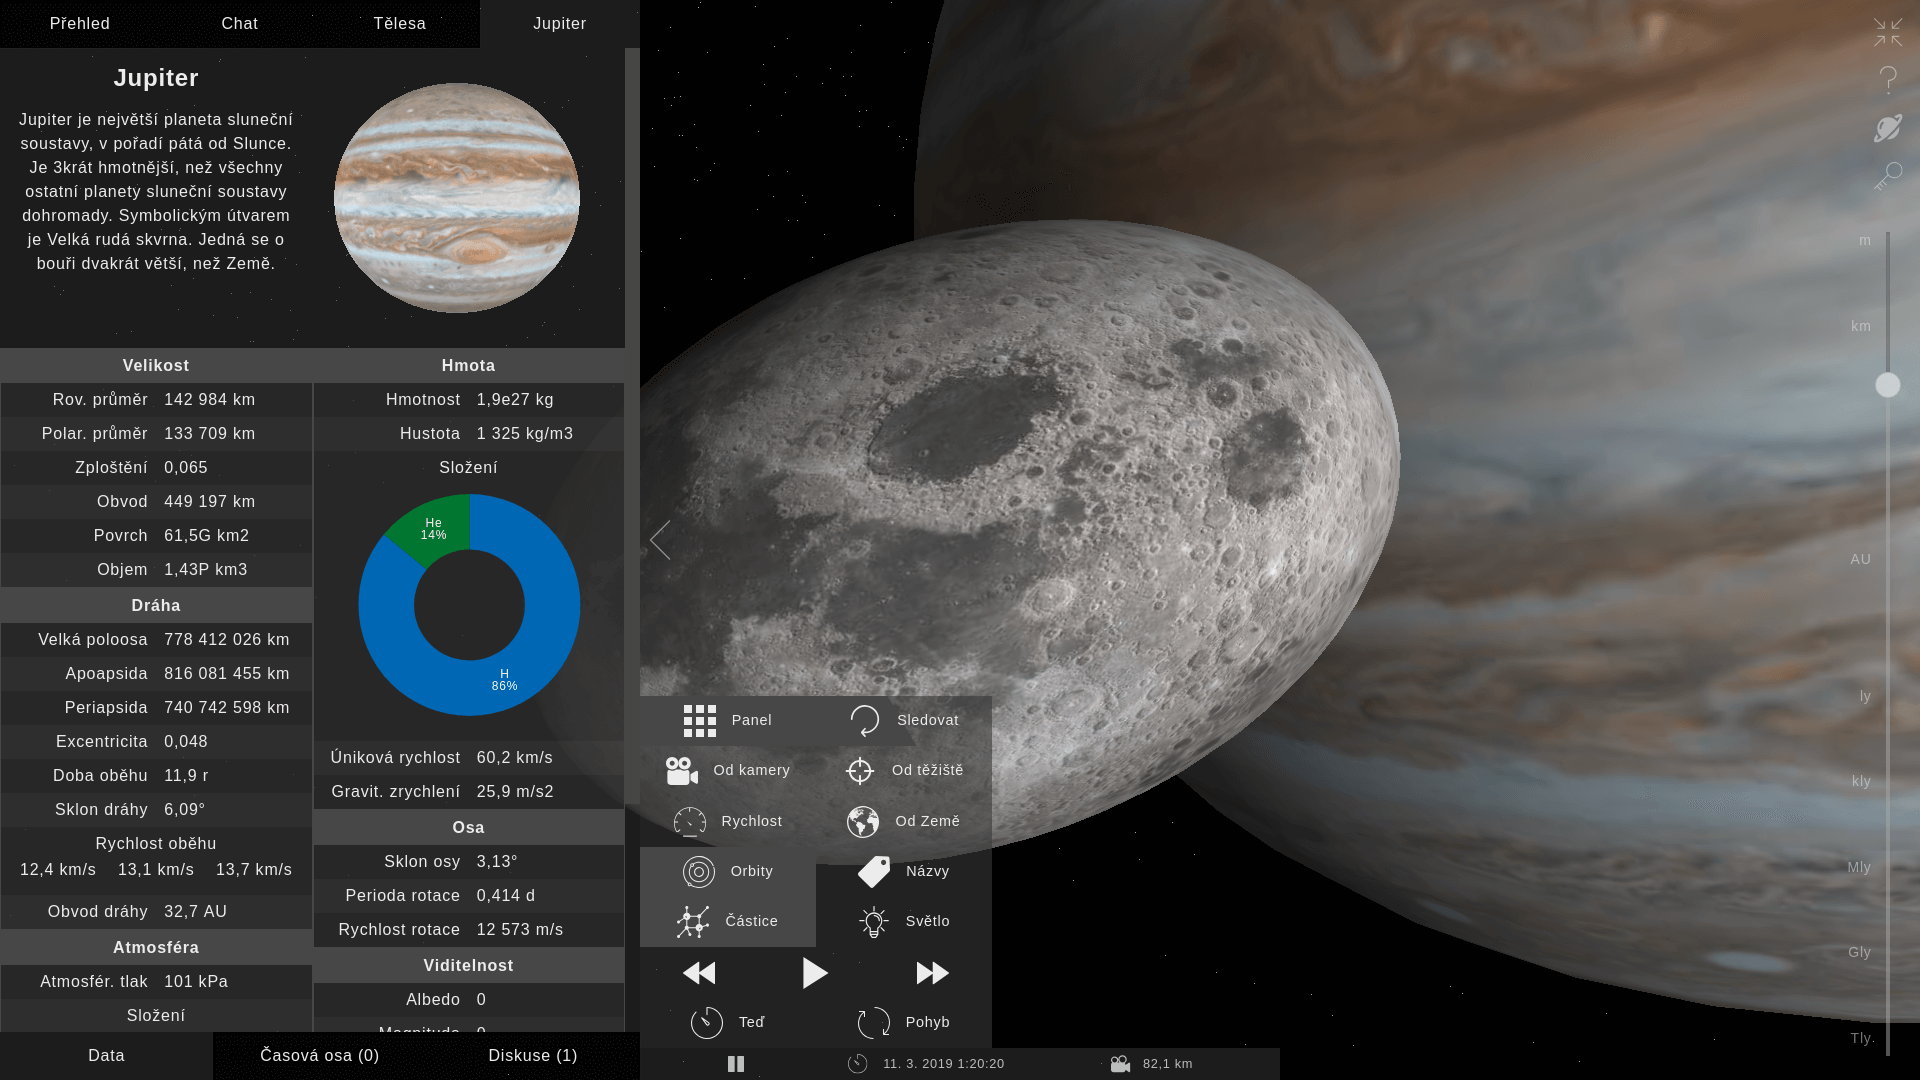
\includegraphics[width=450pt]{Images/Simulator.png}
\caption{Simulátor}
\end{center}
\end{figure}

\vspace*{-1cm}
\subsection{Uživatelský panel}

Uživatelský panel je sekundární okno, ve kterém si uživatel může zobrazovat části aplikace bez nutnosti opouštět aktuální stránku. Zobrazuje se jako poloprůhledný obdélník v levé části obrazovky a~obsahuje 3~nezávislé záložky.

\subsubsection{Přehled}

Výchozí položka v~uživatelském panelu je rozdělena na 2 části. Nalevo se zobrazuje posledních 50 událostí a~zpráv uživatelů. Nachází se zde i~formulář pro napsání nové zprávy. V~případě, že zpráva začíná zavináčem ve tvaru „@uživatel“, bude se jednat o~soukromou zprávu pro dále specifikovaného uživatele. Na pravé straně je pak seznam všech uživatelů, které lze řadit buď podle poslední aktivity nebo podle reputace. Přihlášený uživatel zde také vidí stručné informace o~svém účtu.

\begin{figure}[H]
\begin{center}
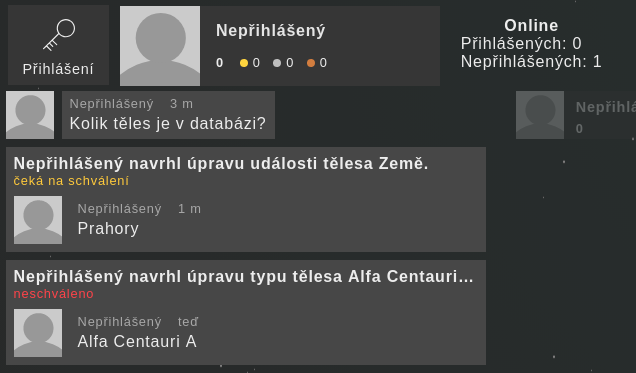
\includegraphics[width=350pt]{Images/Overview.png}
\caption{Přehled}
\end{center}
\end{figure}

\vspace*{-1cm}
\subsubsection{Seznam těles}

Seznam těles umožňuje zobrazit tělesa v~databázi i~s~jejich údaji. Údaje mohou být:

\begin{itemize}
\item \textbf{Absolutní}: Zobrazí absolutní hodnotu (např. průměr Slunce je 1~392~684~km).
\item \textbf{Relativní k libovolnému tělesu}: Zobrazí poměr aktuální hodnoty ku hodnotě u~porovnávaního tělesa (např. průměr Slunce je roven 109~průměrům Země).
\end{itemize}

Tělesa lze řadit vzestupně i~sestupně podle libovolného kritéria a~taktéž je lze podle libovolných kritérií filtrovat za použití následujících vztahů:

\begin{itemize}
\item \textbf{Obsahuje}: Vyhoví, pokud hodnota obsahuje hledaný text.
\item \textbf{Je roven}: Vyhoví, pokud je hodnota rovna hledanému textu.
\item \textbf{Začíná na}: Vyhoví, pokud hodnota začíná hledaným textem.
\item \textbf{Končí na}: Vyhoví, pokud hodnota končí hledaným textem.
\item \textbf{Je větší než}: Vyhoví, pokud je hodnota větší, než hledaný text. V~případě nečíselné hodnoty vyhoví ty, které se v~abecedě nachází později.
\item \textbf{Je menší než}: Vyhoví, pokud je hodnota menší, než hledaný text. V~případě nečíselné hodnoty vyhoví ty, které se v~abecedě nachází dříve.
\end{itemize} 

\begin{figure}[H]
\begin{center}
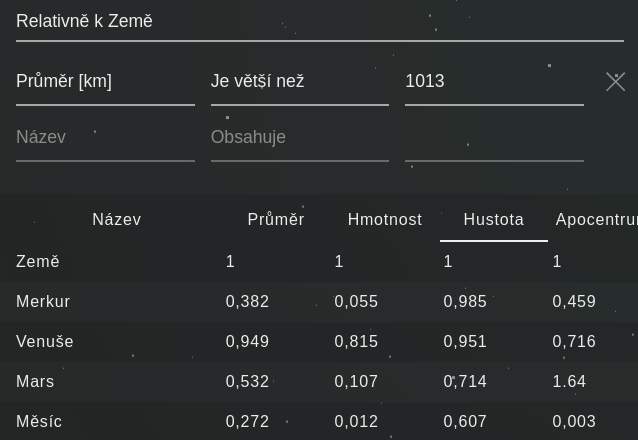
\includegraphics[width=350pt]{Images/Bodies.png}
\caption{Seznam těles}
\end{center}
\end{figure}

\vspace*{-1cm}
\subsubsection{Detail tělesa}

Detail tělesa se skládá ze tří záložek. Výchozí z nich zobrazuje výčet všech známých údajů v~tabulce o~daném tělese. Součástí je i~krátká slovní charakteristika tělesa a~jeho 3D vizualizace.

Na druhé záložce se nachází časová osa, na které jsou vyneseny historické události spojené s~tělesem. Každá událost obsahuje rok, ve kterém nastala, název a~po najetí kurzorem  i~krátký popis. Je zde i stručný graf zobrazující počet výskytů události v~jednotlivých časových obdobích.

Třetí a~poslední záložka je určena pro diskuse. Každý zde může reagovat na již existující diskuse, nebo může založit vlastní vlákno. Všechny příspěvky uživatelů lze kladně nebo záporně hodnotit, v důsledku čehož se bude přičítat nebo odečítat reputace autora.

\begin{figure}[H]
\begin{center}
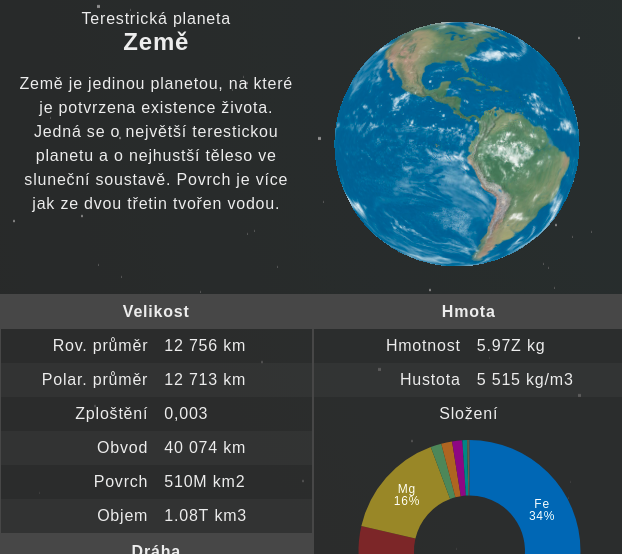
\includegraphics[width=350pt]{Images/Body.png}
\caption{Detail tělesa}
\end{center}
\end{figure}

\begin{figure}[H]
\begin{center}
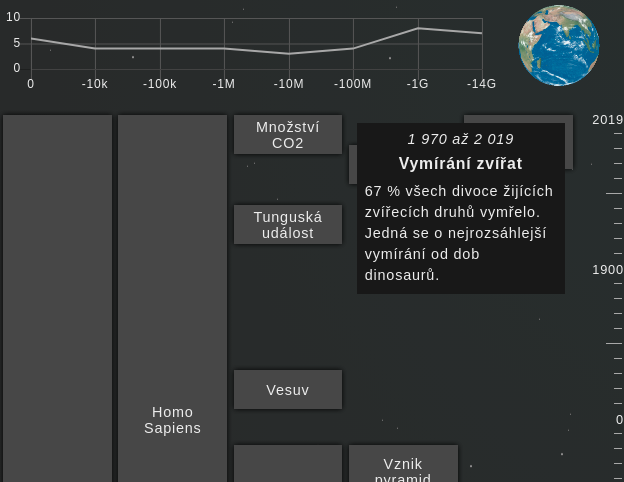
\includegraphics[width=350pt]{Images/Timeline.png}
\caption{Časová osa tělesa}
\end{center}
\end{figure}

\begin{figure}[H]
\begin{center}
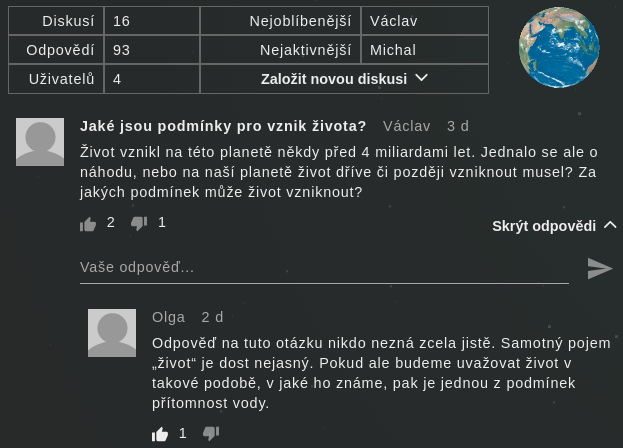
\includegraphics[width=350pt]{Images/Discussion.png}
\caption{Diskuse o tělese}
\end{center}
\end{figure}

\vspace*{-1cm}
\subsection{Podmínky užití}

Tato stránka obsahuje právní ustanovení, která určují, jak mohou potenciální uživatelé zacházet s~aplikací. Píše se zde zejména o~tom, že se na aplikaci vztahují práva a~povinnosti uvedená v~prohlášení autora na začátku tohoto dokumentu. Zároveň jsou zde také uvedeny všechny ty části aplikace, které nevytvořil sám autor a~mohly by se na ně vztahovat další licenční podmínky.

Konkrétně se jedná o~všechny grafické soubory, zejména pak textury těles, které jsou brány ze zdrojů, jež umožňují jejich volné užívání a~ikony. Všechny ikony jsou převzaty z~webu \url{https://www.flaticon.com}, který umožňuje ve standardní edici zdarma využívat ikony za podmínky uvedení autora. Další část aplikace, kterou nevytvořil autor, tvoří balíčky NPM uvedené v~příloze C~na konci tohoto dokumentu. Protože uživatelé mohou přidávat vlastní obsah, je zde uvedeno také zřeknutí se za vše, co uživatelé nahrají.

\section{Problémy řešené při implementaci}

\subsection{Omezení viditelnosti těles}

V~databázi je uloženo velké množství těles. Pokud by se popisky a~dráhy všech těles zobrazovaly najednou, bylo by těžké se v simulátoru orientovat. Navíc by tento stav měl negativní důsledky na výkon aplikace. Proto se ve vykreslovací smyčce počítá relativní poloha všech těles vzhledem ke kameře. V~závislosti na této poloze se určí, jak se bude dané těleso zobrazovat. Může nastat několik případů, které je nutno ošetřit:

\begin{itemize}
\item \textbf{Dráha je 40krát větší/menší než obrazovka}: Dráha tělesa bude poloprůhledná, popisky se nebudou zobrazovat.
\item \textbf{Dráha je 1000krát větší/menší než obrazovka}: Dráha ani popisky se nebudou zobrazovat.
\item \textbf{Vzdálenost od tělesa je 40krát větší než vzdálenost od centrálního tělesa}: Dráha tělesa bude poloprůhledná, popisky se nebudou zobrazovat.
\item \textbf{Vzdálenost od tělesa je 1000krát větší než vzdálenost od centrálního tělesa}: Dráha ani popisky se nebudou zobrazovat.
\end{itemize} 

První dva body řeší případy, kdy je těleso příliš oddálené nebo příliš přiblížené. Poslední dva body řeší situaci, ve které má uživatel sice přiměřené přiblížení kamery, nicméně se od tělesa nachází příliš daleko. Příkladem může být situace, kdy si uživatel prohlíží ze vzdálenosti 400~tisíc km prstence planety Saturn. Dráha zemského Měsíce je přiměřeně velká (406~tisíc km), ale přesto by se neměla vykreslovat. Od Saturnu je totiž vzdálena 1,2~miliardy km.~\cite{rees}

\subsection{Sestavení aplikace a~optimalizace}

\begin{figure}[H]
  \centering
  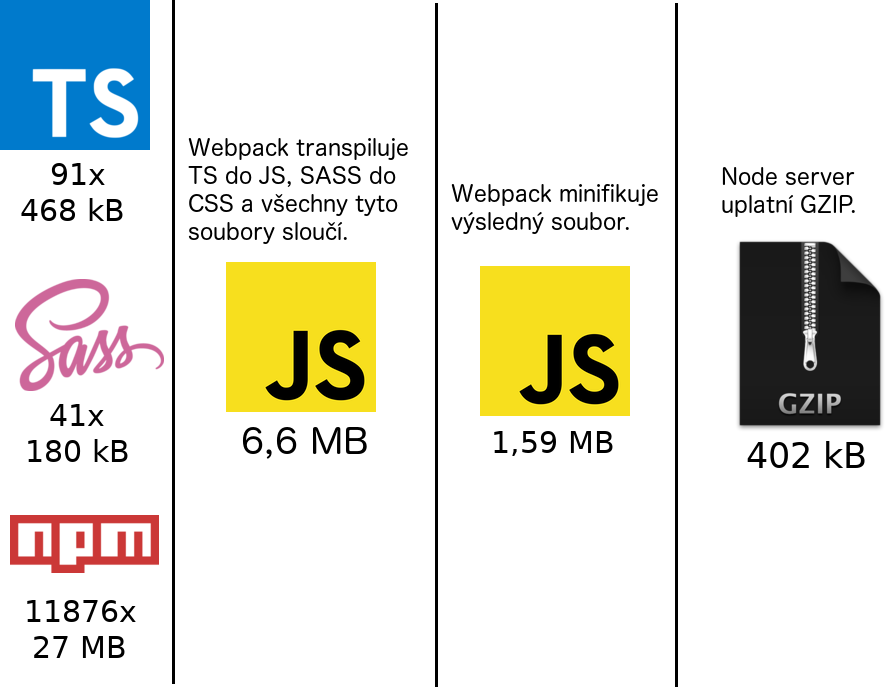
\includegraphics[width=280pt]{Images/Webpack.png}
  \caption[Sestavení aplikace a~optimalizace]{Sestavení aplikace a~optimalizace   \footnotemark[1]\textsuperscript{, }\footnotemark\textsuperscript{, }\footnotemark}
\end{figure}

\footnotetext[1]{Ikona SASS převzata z \url{https://sass-lang.com/assets/img/logos/logo-b6e1ef6e.svg}}
\footnotetext[2]{Ikona NPM převzata z \url{https://pepa.holla.cz/wp-content/uploads/2016/06/npm.png}}
\footnotetext[3]{Ikona GZIP převzata z \url{https://codeopinion.com/wp-content/uploads/2016/02/gzip.png}}

\vspace*{-0.5cm}
\subsubsection{Transpilace a~sloučení JS a~CSS souborů}

V~projektu se nachází velké množství souborů s~typescriptovým kódem a~souborů se styly. Zahajovat HTTP požadavek pokaždé, kdy si uživatel chce stáhnout jakýkoliv z~těchto souborů vyžaduje hodně režije a je to z~hlediska času i~přenesených dat náročné. Je proto výhodnější všechny tyto soubory sloučit do jediného a~ten stáhnout jako jeden celek.

Ze všeho nejdříve je ale nutné transpilovat zdrojové kódy do nativních jazyků. Prohlížeče totiž TypeScriptu ani SASSu nerozumí. TypeScript se transpiluje do JavaScriptu za využití transpilátoru, jenž je dodáván společně s~TypeScriptem. Pro převod SASS na CSS slouží Webpack. Ten následně také všechny takto transpilovaného soubory slouží do jediného javascriptového souboru.

\subsubsection{Minifikace a~komprese GZIP}

I přesto, že jsou všechny zdrojové soubory sloučené do jednoho, stále se jedná o~velký objem dat. Je proto vhodné celý soubor pomocí nástroje Webpack minifikovat~–~odebrat z~něj přebytečné mezery, komentáře a~zkrátit názvy lokálních proměnných.

Pro ještě větší redukci přenesených dat je dobré nastavit Node.js server tak, aby na všechny odeslané soubory uplatnil kompresi GZIP.

\subsection{Bezpečnost a~ochrana dat}

\subsubsection{Autentizace pomocí tokenu}

Uživatel se autentizuje při přihlášení svým emailem a heslem, čímž mu je umožněn přístup na jeho účet. Nicméně uživatele je třeba znovu autentizovat i~během jeho relace po přihlášení, kdykoliv komunikuje se serverem. Tím lze zabezpečit autorizaci a~omezit provádění určitých operací (např. editování tělesa, schvalování úprav, ...) pouze na konkrétní uživatele nebo skupiny uživatelů (např. pouze přihlášení, administrátoři, ...). Nabízí se několik možností v tom, co na server posílat vždy, když je třeba autentifikace:

\begin{itemize}
\item \textbf{Email a heslo}: Nechat uživatele zadávat přihlašovací údaje pokaždé, když je třeba komunikovat se serverem, by bylo obtěžující. A~ukládat heslo na straně klienta není zas bezpečné, protože by zde muselo být v~čitelné podobě.

\item \textbf{ID uživatele}: Jedná se o~nebezpečný postup. ID uživatele je veřejný údaj, ke kterému mají přístup i~všichni ostatní. Nic by nebránilo útočníkovi poslat \textit{HTTP} požadavek s~ID libovolného uživatele.

\item \textbf{Token}: Ideálním způsobem se zdá být vygenerování pseudonáhodného textového řetězce při přihlášení. Tímto řetězcem se po dobu přihlášení bude uživatel prokazovat. Protože tento řetězec nezná nikdo jiný, než uživatel sám, nikdo jiný se s~ním nemůže autentizovat. Navíc proti zneužití má omezenou platnost, po jejímž vypršení je třeba požádat o~nový token.
\end{itemize}

V~aplikaci je využit poslední ze zmíněných způsobů. Token má platnost 30 minut a~je zajištěna bezpečná autoritace. Každý může provádět pouze ty operace, na které má skutečně právo.

\subsubsection{Hashování hesel}

Ukládat hesla v čitelné podobě do databáze není bezpečné. Potenciální útočník, který by prolomil zabezpečení serveru a~dostal se k~databázi by viděl hesla všech uživatelů. Tento problém řeší \textit{hashování hesel}.

Do databáze se neuloží heslo samotné, ale pouze jeho otisk (\textit{hash}). Když je potřeba porovnat zadané heslo (např. při přihlášování) s heslem, porovnají se jejich otisky. Tím je umožněna autentifikace a~zároveň je znemožněno útočníkovi přečíst hesla z~databáze.

Pro vyšší bezpečnost se otisk nevypočítává z pouhého hesla, ale hesla spojeného s~dalším nijak nesouvisejícícm řetězcem. Tím se zabrání možnosti, aby více uživatelů mělo stejné heshe, pokud mají stejná hesla. Tomuto dodatečnému řetězci se říká sůl (\textit{salt}). Často se také otisk vypočítává několikrát za sebou, takže v databázi není uložen otisk hesla, ale otisk, který vznikl na základě jiného otisku.

\textit{Hash} je výsledkem jednosměrné funkce. To znamená, že z již vypočteného hashe nelze získat původní text. Výjimku tvoří zastaralé \textit{hashovací} funkce, které již byly prolomeny. Je vytvořena databáze pro všechny možné otisky a~texty, ze kterých byly vypočítány.

V~aplikaci je použita \textit{hashovací funkce bcrypt} s~10 iteracemi a~to přímo na úrovni databáze. Celá logika je skryta do tzv. \textit{Mongoose pluginu}. Ten může reagovat na různé události a~modifikovat dokument.

\lstinputlisting[caption={Hashování hesel v Mongoose schématu}, language={JavaScript}]{SourceCodes/Hash.js}

\vspace*{-0.5cm}
\subsection{Zobrazování hodnot fyzikálních veličin}

Aplikace zobrazuje různě velké hodnoty různých fyzikálních veličin. Z~důvodu přehlednosti a~omezeného množství prostoru, ve kterém se tyto hodnoty zobrazují, byla vytvořena pomocná třída \code{Units} umístěná do modulu \code{Utils}. Ta umožňuje převádět a~formátovat jednotky do několika podob.

\lstinputlisting[caption={Ukázka formátování jednotek}, language={JavaScript}]{SourceCodes/Units.js}

Všechny číselné hodnoty se automaticky zaokrouhlují s~rozumnou přesností:

\lstinputlisting[caption={Ukázka zaokrouhlování hodnot}, language={JavaScript}]{SourceCodes/Round.js}

Není nutné používat předdefinované jednotky v~této třídě a~lze si vytvořit vlastní. Vytvoření jednotek pro velikost vypadá takto:

\lstinputlisting[caption={Tvorba vlastních jednotek}, language={JavaScript}]{SourceCodes/CreateUnits.js}

\vspace*{-0.5cm}
\subsection{Vykreslování časové osy}

Pro vykreslení časové osy představené v~podkapitole \textit{4.5.3~Detail tělesa} byla v~rámci projektu vytvořena komponenta \textit{EventsArea}. Ta umožňuje vykreslit pole událostí na \textit{2D} ploše v~podobě čtyřúhelníků tak, aby si souřadnice jednotlivých událostí odpovídaly. V~případě časové osy jsou těmito souřadnicemi počáteční a~koncový rok události.

Situace je o~to komplikovanější, že časová osa nemusí být lineární a~dokonce ani logaritmická. Komponenta proto na vstupu vedle pole událostí přijme i~pole hraničních souřadnic. Díky tomu je možné zobrazit roky 2019 až 0 jako jeden díl na časové ose a~o~něco níže naprosto stejný díl pro roky -1 až -10~000, stejně jako např. -5~mld. až -10~mld.

Překrývání jednotlivých události je ošetřeno tak, že se vykreslí do různých sloupců. Je také možno nastavit počet mezistupňů mezi hraničními souřadnicemi. Ty lze nastylovat např. jako čáry na pravítku pro zlepšení přehlednosti. Při pohybu s kurzorem myši nad oblastí se zobrazuje horizontální čára s aktuální souřadnicí (rokem), nad kterou se kurzor nachází. Pro implementaci komponenty byla použita \textit{CSS} vlastnost \textit{grid}.

\lstinputlisting[caption={Příklad použití komponenty EventsArea}, language={JavaScript}]{SourceCodes/EventsArea.js}


%%%%%%%%%%%%%%%%%%%%%%%%%%%%%%%%%%%%%%%%%%%%%%%%%%%%%%%%%%%%
% ZÁVĚR
%%%%%%%%%%%%%%%%%%%%%%%%%%%%%%%%%%%%%%%%%%%%%%%%%%%%%%%%%%%%

\clearpage \phantomsection \addcontentsline{toc}{section}{Závěr}
\section*{Závěr}


%%%%%%%%%%%%%%%%%%%%%%%%%%%%%%%%%%%%%%%%%%%%%%%%%%%%%%%%%%%%
% POUŽITÁ LITERATURA
%%%%%%%%%%%%%%%%%%%%%%%%%%%%%%%%%%%%%%%%%%%%%%%%%%%%%%%%%%%%

\clearpage \phantomsection \addcontentsline{toc}{section}{\refname}

\begin{thebibliography}{99}	% parametr určuje nejširší položku

% nezlomitelné spojovníky lze zapisovat zkratkou "- nebo příkazem \babelhyphen{nobreak}

\bibitem{aggregation}
Aggregate.
\textit{mongoose.} [online]. [cit.\,22.~2.~2019].
Dostupné z: {\ttfamily \url{https://mongoosejs.com/docs/api.html#Aggregate}}.

\bibitem{reactbook}
BANKS, Alex, PORCELLO, Eve. Learning React: functional web development with React and Redux. Sebastopol, CA: O'Reilly Media, 2017 [cit. 25. 10. 2018]. ISBN: 978-1-4919-5462-1.

\bibitem{webpack}
Concepts.
\textit{webpack.} [online]. [cit.\,22.~2.~2019].
Dostupné z: {\ttfamily \url{https://webpack.js.org/concepts}}.

\bibitem{graphic}
ECK, David. \textit{Introduction to Computer Graphics.} [online]. Version 1.2, January 2018. [cit.\,22.~2.~2019]. Dostupné z \url{http://math.hws.edu/eck/cs424/downloads/graphicsbook-linked.pdf}.

\bibitem{jsconcat}
Fantastic front-end performance.
\textit{HACKS.} [online]. 20~2~2019. [cit.\,22.~2.~2019].
Dostupné z: {\ttfamily \url{https://hacks.mozilla.org/2012/12/fantastic-front-end-performance-part-1-concatenate-compress-cache-a-node-js-holiday-season-part-4/}}.

\bibitem{filestructure}
File Structure.
\textit{React.} [online]. [cit.\,22.~2.~2019].
Dostupné z:\newline{\ttfamily \url{https://reactjs.org/docs/faq-structure.html}}.

\bibitem{swaggerui}
JOHNSON, Tom. Swagger UI tutorial. \textit{Documenting APIs.}. [online]. c2019 [cit.\,22.~2.~2019]. Dostupné z: {\ttfamily \url{https://idratherbewriting.com/learnapidoc/pubapis_swagger.html}}

\bibitem{jpl}
JPL Solar System Dynamics. \textit{JPL Solar System Dynamics} [online]. [cit. 25. 10. 2018] Dostupné z: \url{https://ssd.jpl.nasa.gov}..

\bibitem{simulations}
KAVIČKA, Antonín. Pardubice. Elektronické sylaby přednášek předmětu Modelování a~simulace. [cit.\,22.~2.~2019].

\bibitem{kleczek}
KLECZEK, Josip. Velká encyklopedie vesmíru. Praha: Academia, 2002s [cit. 25. 10. 2018]. ISBN 80-200-0906-x.

\bibitem{nodebook}
MARDAN, Azat. Practical Node.js: building real-world scalable web apps. Berkeley, California: Apress, [2014]. Expert‘s voice in Web development. ISBN 978-1-4302- 6595-5.

\bibitem{node}
MROZEK, Jakub. JavaScript na serveru: Architektura a první Hello World.
\textit{Zdroják.} [online]. 5.~10.~2012. [cit.\,22.~2.~2019].  ISSN 1803-5620.
Dostupné\newline z:~{\ttfamily \url{https://www.zdrojak.cz/clanky/javascript-na-serveru-architektura-a-prvni-hello-world/}}.

\bibitem{mongomongoose}
MROZEK, Jakub. JavaScript na serveru: MongoDB, Mongoose a AngularJS.
\textit{Zdroják.} [online]. 26.~10.~2012. [cit.\,22.~2.~2019]. ISSN 1803-5620.
Dostupné z:\newline{\ttfamily \url{https://www.zdrojak.cz/clanky/javascript-na-serveru-mongodb-mongoose-angularjs}}.

\bibitem{emulations}
PETERKA, Jiří. Simulace vs. emulace. \textit{earchiv.cz}. [online]. 1992. [cit.~22.~2.~2019]. Dostupné z:~{\ttfamily\url{http://www.earchiv.cz/a92/a210c120.php3}}.

\bibitem{rees}
REES, Martin, Vesmír. Přeložil Pavel PŘÍHODA. Praha: Knižní klub, 2006 [cit. 25. 10. 2018]. ISBN 80-242-1668-x.

\bibitem{michalrepik}
ŘEPÍK, Michal. Keplerova rovnice. \textit{Michal Řepík}. [online]. 22.~12.~2014. [cit. 16.~3.~2019]. Dostupné z:~{\ttfamily\url{http://www.michalrepik.cz/matematika/keplerova_rovnice.html}}.

\bibitem{sass}
Sass Basics.
\textit{Sass.} [online]. [cit.\,22.~2.~2019].
Dostupné z:\newline{\ttfamily \url{https://sass-lang.com/guide}}.

\bibitem{onewaydatabinding}
Thinking in React.
\textit{React.} [online]. [cit.\,22.~2.~2019]. 
Dostupné\newline z:~{\ttfamily \url{https://reactjs.org/docs/thinking-in-react.html}}.

\bibitem{typescript}
TypeScript. 
\textit{TypeScript.} [online]. [cit.\,22.~2~2019]. 
Dostupné\newline z:~{\ttfamily \url{https://www.typescriptlang.org}}.

\bibitem{git}
Úvod - Základy systému Git.
\textit{git.} [online]. [cit.\,22.~2.~2019]. 
Dostupné z: {\ttfamily \url{https://git-scm.com/book/cs/v1/%C3%9Avod-Z%C3%A1klady-syst%C3%A9mu-Git}}.



\end{thebibliography}


%%%%%%%%%%%%%%%%%%%%%%%%%%%%%%%%%%%%%%%%%%%%%%%%%%%%%%%%%%%%
% PŘÍLOHY
%%%%%%%%%%%%%%%%%%%%%%%%%%%%%%%%%%%%%%%%%%%%%%%%%%%%%%%%%%%%


\clearpage \phantomsection \addcontentsline{toc}{section}{Seznam příloh}
\section*{Seznam příloh}

\noindent Příloha~A -- Struktura databáze \dotfill \pageref{prilohaA}

\noindent Příloha~B -- Využití aggregation frameworku \dotfill \pageref{prilohaB}

\noindent Příloha~C -- Externí balíčky NPM použité v aplikaci \dotfill \pageref{prilohaC}

\noindent Příloha~D -- Seznam souborů zdrojových kódů na přiloženém nosiči \dotfill \pageref{prilohaD}

\clearpage \phantomsection\label{prilohaA} 

% do obsahu i do záložek PDF:
%\addcontentsline{toc}{section}{Příloha~A -- Uvozovky}
% pouze do záložek PDF:
%\pdfbookmark[1]{Příloha~A -- Struktura databáze}{prilohaA}	% záložka do 
%\addcontentsline{toc}{section}{Příloha~A -- Struktura databáze}
\section*{Příloha~A --  Struktura databáze}
%\pdfbookmark[1]{Příloha~B -- Využití aggregation frameworku}{prilohaB}	% záložka do PDF

\begin{figure}[H]
\vspace{-0.5cm}\hspace{-1cm}
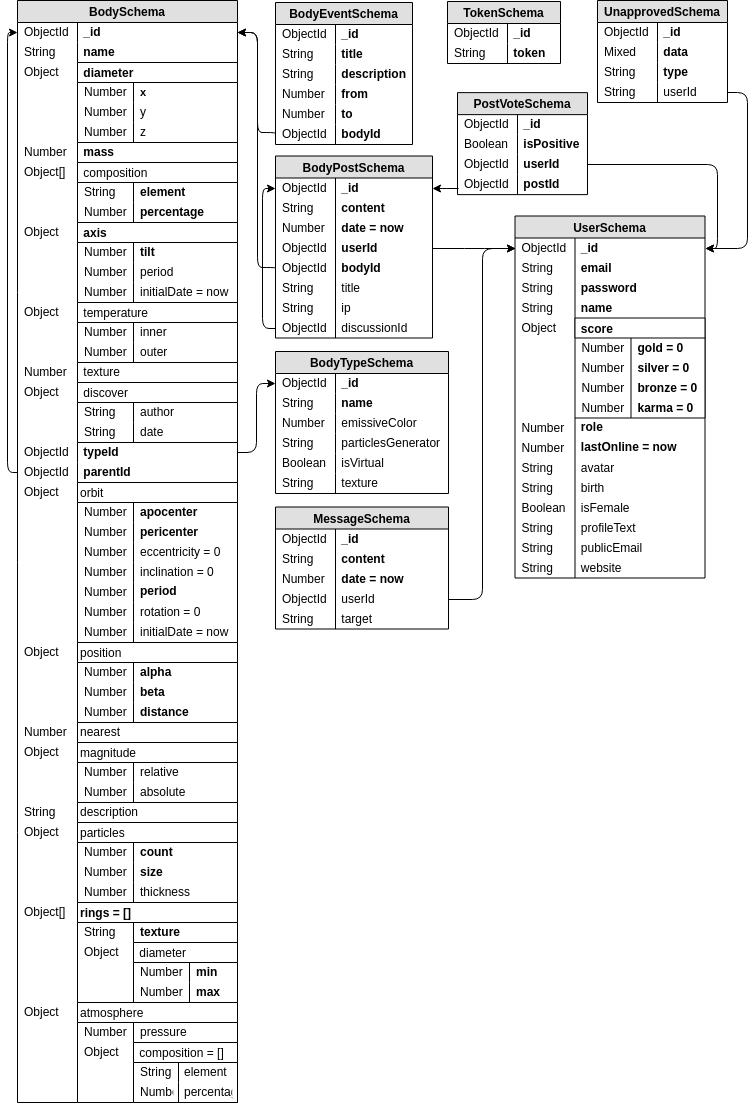
\includegraphics[width=450pt]{Images/DB.png}
\end{figure}

\clearpage \phantomsection\label{prilohaB} 

%\addcontentsline{toc}{section}{Příloha~B -- Využití aggregation frameworku}
\section*{Příloha~B --  Využití aggregation\newline frameworku}

\lstinputlisting[nolol,language={JavaScript}]{SourceCodes/Aggregation.js}

\clearpage \phantomsection\label{prilohaC} 

%\addcontentsline{toc}{section}{Příloha~C -- Externí balíčky NPM použité v aplikaci}
\section*{Příloha~C --  Externí balíčky NPM\newline použité v aplikaci}

\subsection*{Backend}

\begin{code}
bcrypt \textasciicircum2.0.1\newline
body-parser \textasciicircum1.18.3\newline
compression \textasciicircum1.7.2\newline
express \textasciicircum4.16.3 (@types/express \textasciicircum4.16.1)\newline
express-openapi \textasciicircum1.10.0\newline
http-status-codes \textasciicircum1.3.0\newline
jsonwebtoken \textasciicircum8.3.0 (@types/jsonwebtoken \textasciicircum8.3.2)\newline
mongoose \textasciicircum5.4.11 (@types/mongoose \textasciicircum5.3.21) \newline
path \textasciicircum0.12.7\newline
swagger-ui-express \textasciicircum3.0.10\newline
nodemon \textasciicircum1.17.15\newline
npm-run-all \textasciicircum4.1.3
\end{code}

\subsection*{Frontend}

\begin{code}
axios \textasciicircum0.18.0\newline
chart.js \textasciicircum2.7.3\newline
chartjs-plugin-labels \textasciicircum1.1.0\newline
classnames \textasciicircum2.2.6\newline
js-cookie \textasciicircum2.2.0 (@types/js-cookie \textasciicircum2.2.0)\newline
node-sass \textasciicircum4.9.3\newline
path \textasciicircum0.12.7\newline
react \textasciicircum16.5.2 (@types/react \textasciicircum16.8.7)\newline
react-chartjs-2 \textasciicircum2.7.4\newline
react-dom \textasciicircum16.5.2 (@types/react-dom \textasciicircum16.0.8)\newline
react-rangeslider \textasciicircum2.2.0\newline
react-redux \textasciicircum5.0.7 (@types/react-redux \textasciicircum5.0.21)\newline
react-router-dom \textasciicircum4.3.1 (@types/react-router-dom \textasciicircum4.3.1)\newline
redux-form \textasciicircum7.4.2 (@types/redux-form \textasciicircum7.4.8)\newline
redux-thunk \textasciicircum2.2.0\newline
screenfull \textasciicircum3.3.3\newline
three \textasciicircum0.94.0 (@types/three \textasciicircum0.92.24)\newline
three-trackballcontrols \textasciicircum0.0.7\newline
css-loader \textasciicircum0.28.9\newline
postcss-loader \textasciicircum2.1.6\newline
sass-loader \textasciicircum6.0.6\newline
style-loader \textasciicircum0.20.2\newline
ts-loader \textasciicircum5.2.1\newline
typescript \textasciicircum3.1.1\newline
webpack \textasciicircum4.20.2\newline
webpack-cli \textasciicircum3.1.2\newline
webpack-dev-server \textasciicircum3.1.9 (@types/webpack-dev-server \textasciicircum2.9.6)
\end{code}

\clearpage \phantomsection\label{prilohaD} 

%\addcontentsline{toc}{section}{Příloha~D -- Seznam souborů zdrojových kódů na přiloženém nosiči}
\section*{Příloha~D --  Seznam souborů zdrojových kódů na přiloženém nosiči}

.gitignore\newline package-lock.json\newline package.json\newline src/Client/package-lock.json\newline src/Client/package.json\newline src/Client/postcss.config.js\newline src/Client/src/Charts/Components/DonutChart.tsx\newline src/Client/src/Charts/Components/LineChart.tsx\newline src/Client/src/Charts/index.ts\newline src/Client/src/Controls/Components/AboutControl.tsx\newline src/Client/src/Controls/Components/Alert.tsx\newline src/Client/src/Controls/Components/AuthenticationControl.tsx\newline src/Client/src/Controls/Components/ContextInfo.tsx\newline src/Client/src/Controls/Components/ContextMenu.tsx\newline src/Client/src/Controls/Components/ContextTrigger.tsx\newline src/Client/src/Controls/Components/Control.tsx\newline src/Client/src/Controls/Components/ControlLink.tsx\newline src/Client/src/Controls/Components/ControlPanel.tsx\newline src/Client/src/Controls/Components/FullScreenControl.tsx\newline src/Client/src/Controls/Components/HelpControl.tsx\newline src/Client/src/Controls/Components/HomeControl.tsx\newline src/Client/src/Controls/Components/UIControl.tsx\newline src/Client/src/Controls/Components/ViewSizeControl.tsx\newline src/Client/src/Controls/Styles/Alert.scss\newline src/Client/src/Controls/Styles/Context.scss\newline src/Client/src/Controls/Styles/ContextInfo.scss\newline src/Client/src/Controls/Styles/ControlPanel.scss\newline src/Client/src/Controls/Styles/Controls.scss\newline src/Client/src/Controls/index.scss\newline src/Client/src/Controls/index.ts\newline src/Client/src/Forms/Components/Back.tsx\newline src/Client/src/Forms/Components/Field.tsx\newline src/Client/src/Forms/Components/FlexRow.tsx\newline src/Client/src/Forms/Components/Form.tsx\newline src/Client/src/Forms/Components/Note.tsx\newline src/Client/src/Forms/Components/Select.tsx\newline src/Client/src/Forms/Components/Submit.tsx\newline src/Client/src/Forms/Components/Title.tsx\newline src/Client/src/Forms/index.scss\newline src/Client/src/Forms/index.ts\newline src/Client/src/Global/IBodyContrainer.ts\newline src/Client/src/Global/IFilter.ts\newline src/Client/src/Global/ILinkButton.ts\newline src/Client/src/Global/IScene.ts\newline src/Client/src/Global/IStrings.ts\newline src/Client/src/Global/IUniverse.ts\newline src/Client/src/Global/IUserScore.ts\newline src/Client/src/Global/Redux.ts\newline src/Client/src/Global/Select.ts\newline src/Client/src/Global/Table.ts\newline src/Client/src/Global/Units.ts\newline src/Client/src/Panel/Components/AnswerForm.tsx\newline src/Client/src/Panel/Components/Bodies.tsx\newline src/Client/src/Panel/Components/BodiesFilterForm.tsx\newline src/Client/src/Panel/Components/BodiesSettingsForm.tsx\newline src/Client/src/Panel/Components/Body.tsx\newline src/Client/src/Panel/Components/BodyData.tsx\newline src/Client/src/Panel/Components/BodyDiscussion.tsx\newline src/Client/src/Panel/Components/BodyPost.tsx\newline src/Client/src/Panel/Components/BodyTimeline.tsx\newline src/Client/src/Panel/Components/Chat.tsx\newline src/Client/src/Panel/Components/DiscussionForm.tsx\newline src/Client/src/Panel/Components/Overview.tsx\newline src/Client/src/Panel/Components/Panel.tsx\newline src/Client/src/Panel/Redux/ActionTypes.ts\newline src/Client/src/Panel/Redux/PanelActions.ts\newline src/Client/src/Panel/Redux/PanelReducer.ts\newline src/Client/src/Panel/Styles/Bodies.scss\newline src/Client/src/Panel/Styles/Body.scss\newline src/Client/src/Panel/Styles/Chat.scss\newline src/Client/src/Panel/Styles/Overview.scss\newline src/Client/src/Panel/Styles/Panel.scss\newline src/Client/src/Panel/index.scss\newline src/Client/src/Panel/index.tsx\newline src/Client/src/System/Components/AnimatedBackground.tsx\newline src/Client/src/System/Components/App.tsx\newline src/Client/src/System/Constants/Strings.ts\newline src/Client/src/System/Redux/ActionTypes.ts\newline src/Client/src/System/Redux/Store.ts\newline src/Client/src/System/Redux/SystemActions.ts\newline src/Client/src/System/Redux/SystemReducer.ts\newline src/Client/src/System/Styles/AnimatedBackground.scss\newline src/Client/src/System/Styles/Home.scss\newline src/Client/src/System/Views/HomeView.tsx\newline src/Client/src/System/index.scss\newline src/Client/src/System/index.ts\newline src/Client/src/Universe/Components/BodyPreview.tsx\newline src/Client/src/Universe/Components/Canvas.tsx\newline src/Client/src/Universe/Components/ControlBar.tsx\newline src/Client/src/Universe/Components/ControlPanel.tsx\newline src/Client/src/Universe/Components/UI.tsx\newline src/Client/src/Universe/Constants/Config.ts\newline src/Client/src/Universe/Constants/Keys.ts\newline src/Client/src/Universe/Constants/Visibility.ts\newline src/Client/src/Universe/Redux/ActionTypes.ts\newline src/Client/src/Universe/Redux/UniverseActions.ts\newline src/Client/src/Universe/Redux/UniverseReducer.ts\newline src/Client/src/Universe/Styles/ControlBar.scss\newline src/Client/src/Universe/Styles/Controls.scss\newline src/Client/src/Universe/Styles/UI.scss\newline src/Client/src/Universe/Utils/BodyContainer.ts\newline src/Client/src/Universe/Utils/BodyFactory.ts\newline src/Client/src/Universe/Utils/Listener.ts\newline src/Client/src/Universe/Utils/Scene.ts\newline src/Client/src/Universe/Utils/TextureStore.ts\newline src/Client/src/Universe/Utils/Universe.ts\newline src/Client/src/Universe/Views/UniverseView.tsx\newline src/Client/src/Universe/index.scss\newline src/Client/src/Universe/index.ts\newline src/Client/src/User/Components/IdentityForm.tsx\newline src/Client/src/User/Components/LoginForm.tsx\newline src/Client/src/User/Components/SignUpForm.tsx\newline src/Client/src/User/Components/UserInfo.tsx\newline src/Client/src/User/Components/UsersList.tsx\newline src/Client/src/User/Redux/ActionTypes.ts\newline src/Client/src/User/Redux/UserActions.ts\newline src/Client/src/User/Redux/UserReducer.ts\newline src/Client/src/User/Styles/UserInfo.scss\newline src/Client/src/User/Views/IdentityView.tsx\newline src/Client/src/User/Views/LoginView.tsx\newline src/Client/src/User/Views/SignUpView.tsx\newline src/Client/src/User/index.scss\newline src/Client/src/User/index.ts\newline src/Client/src/Utils/Components/AsyncEntity.tsx\newline src/Client/src/Utils/Components/BlurLayout.tsx\newline src/Client/src/Utils/Components/Component.tsx\newline src/Client/src/Utils/Components/DataTable.tsx\newline src/Client/src/Utils/Components/Dropdown.tsx\newline src/Client/src/Utils/Components/EventsArea.tsx\newline src/Client/src/Utils/Components/FadeLayout.tsx\newline src/Client/src/Utils/Components/Link.tsx\newline src/Client/src/Utils/Components/Loader.tsx\newline src/Client/src/Utils/Components/Menu.tsx\newline src/Client/src/Utils/Components/QueryMenu.tsx\newline src/Client/src/Utils/Components/RelativeTime.tsx\newline src/Client/src/Utils/Components/SimpleComponent.tsx\newline src/Client/src/Utils/Components/StatelessComponent.tsx\newline src/Client/src/Utils/Components/Table.tsx\newline src/Client/src/Utils/Components/ToggleLayout.tsx\newline src/Client/src/Utils/Components/UILayout.tsx\newline src/Client/src/Utils/Components/View.tsx\newline src/Client/src/Utils/Constants/Config.ts\newline src/Client/src/Utils/Constants/CookieExpirations.ts\newline src/Client/src/Utils/Constants/Cookies.ts\newline src/Client/src/Utils/Constants/Queries.ts\newline src/Client/src/Utils/Constants/Titles.ts\newline src/Client/src/Utils/Constants/Urls.ts\newline src/Client/src/Utils/Styles/BlurLayout.scss\newline src/Client/src/Utils/Styles/Constants.scss\newline src/Client/src/Utils/Styles/DataTable.scss\newline src/Client/src/Utils/Styles/Default.scss\newline src/Client/src/Utils/Styles/Dropdown.scss\newline src/Client/src/Utils/Styles/EventsArea.scss\newline src/Client/src/Utils/Styles/Loader.scss\newline src/Client/src/Utils/Styles/Table.scss\newline src/Client/src/Utils/Styles/ToggleLayout.scss\newline src/Client/src/Utils/Styles/Utils.scss\newline src/Client/src/Utils/Utils/Cookies.ts\newline src/Client/src/Utils/Utils/Dates.ts\newline src/Client/src/Utils/Utils/Filter.ts\newline src/Client/src/Utils/Utils/Html.ts\newline src/Client/src/Utils/Utils/Redux.ts\newline src/Client/src/Utils/Utils/Request.ts\newline src/Client/src/Utils/Utils/Units.ts\newline src/Client/src/Utils/Utils/Url.ts\newline src/Client/src/Utils/index.scss\newline src/Client/src/Utils/index.ts\newline src/Client/src/index.scss\newline src/Client/src/index.tsx\newline src/Client/webpack.config.js\newline src/Constants/Config.ts\newline src/Constants/DatabaseModels.ts\newline src/Constants/Errors.ts\newline src/Constants/NotificationSubjects.ts\newline src/Constants/Operations.ts\newline src/Constants/index.ts\newline src/Controllers/bodies.ts\newline src/Controllers/bodies/count.ts\newline src/Controllers/bodies/events/{eventId}.ts\newline src/Controllers/bodies/{bodyId}.ts\newline src/Controllers/bodies/{bodyId}/count.ts\newline src/Controllers/bodies/{bodyId}/events.ts\newline src/Controllers/bodies/{bodyId}/posts.ts\newline src/Controllers/bodyTypes.ts\newline src/Controllers/bodyTypes/count.ts\newline src/Controllers/bodyTypes/{bodyTypeId}.ts\newline src/Controllers/login.ts\newline src/Controllers/messages.ts\newline src/Controllers/posts/votes/{voteId}.ts\newline src/Controllers/posts/{postId}/posts.ts\newline src/Controllers/posts/{postId}/votes.ts\newline src/Controllers/users.ts\newline src/Controllers/users/count.ts\newline src/Controllers/users/{userId}.ts\newline src/Database/Database.ts\newline src/Database/DatabaseModel.ts\newline src/Database/Plugins/FillBodyPlugin.ts\newline src/Database/Plugins/HashPlugin.ts\newline src/Database/Plugins/ModifyPlugin.ts\newline src/Database/Schemas/BodyEventSchema.ts\newline src/Database/Schemas/BodyPostSchema.ts\newline src/Database/Schemas/BodySchema.ts\newline src/Database/Schemas/BodyTypeSchema.ts\newline src/Database/Schemas/MessageSchema.ts\newline src/Database/Schemas/PostVoteSchema.ts\newline src/Database/Schemas/TokenSchema.ts\newline src/Database/Schemas/UnapprovedSchema.ts\newline src/Database/Schemas/UserSchema.ts\newline src/Global/Database.ts\newline src/Global/Discussion.ts\newline src/Global/Error.ts\newline src/Global/Event.ts\newline src/Global/FunctionalInterfaces.ts\newline src/Global/Functions.ts\newline src/Global/IBody.ts\newline src/Global/IBodyType.ts\newline src/Global/IFactory.ts\newline src/Global/IObject.ts\newline src/Global/ISecurityModel.ts\newline src/Global/IServer.ts\newline src/Global/IUser.ts\newline src/Global/Item.ts\newline src/Global/Message.ts\newline src/Global/Routes.ts\newline src/Global/Structures.ts\newline src/Global/Universe.ts\newline src/Global/User.tsx\newline src/Models/BodyEventModel.ts\newline src/Models/BodyModel.ts\newline src/Models/BodyPostModel.ts\newline src/Models/BodyTypeModel.ts\newline src/Models/ItemModel.ts\newline src/Models/Model.ts\newline src/Models/MessagesModel.ts\newline src/Models/PostVoteModel.ts\newline src/Models/SecurityModel.ts\newline src/Models/UserModel.ts\newline src/Public/index.html\newline src/Server.ts\newline src/Swagger.ts\newline src/Utils/Arrays.ts\newline src/Utils/Dates.ts\newline src/Utils/Physics.ts\newline src/Utils/Route.ts\newline src/Utils/Security.ts\newline src/Utils/Strings.ts\newline src/index.ts\newline tsconfig.json\newline


%%%%%%%%%%%%%%%%%%%%%%%%%%%%%%%%%%%%%%%%%%%%%%%%%%%%%%%%%%%%
% KONEC DOKUMENTU
%%%%%%%%%%%%%%%%%%%%%%%%%%%%%%%%%%%%%%%%%%%%%%%%%%%%%%%%%%%%

\end{document}

% vim:sw=8:ts=8
% EOF
